\cleardoublepage
\chapter[Band structures of semiconductors and insulators]{Band structures of semiconductors\break and insulators\label{ch:band-structures}}
In this chapter we discuss the details of practical calculations, and the results obtained for a manifold of reference insulating materials. Thanks to the validity of Bloch's theorem, discussed in \cref{ch:koopmans-periodic}, it is possible to obtain electronic band structures -- within the primitive cell's BZ -- either from a supercell approach, by means of an unfolding method, or from the primitive cell implementation described in \cref{sec:koopmans-pbc}. The computational details of the calculations, including the description of the unfolding method and of the Koopmans workflow, are discussed in \cref{sec:calculations-koopmans}, while in \cref{sec:results-bands} we report the obtained results.

Some extracts of this chapter, as well as the reported results, have been published in scientific journals \cite{de_gennaro_blochs_2022,colonna_koopmans_2022}.

\clearpage
\section{Calculations with Koopmans functionals\label{sec:calculations-koopmans}}
Electronic-structure calculations using Koopmans spectral functionals are performed following two different approaches, based on the two strategies to compute the screening parameters discussed in \cref{sec:screening-parameters}: the first makes use of the finite energy differences strategy and relies on the SC method to model the system deprived of a particle, the second resorts to linear response theory and takes full advantage of the system's symmetries by exploiting the Wannier-like nature of the variational orbitals. The two approaches have different implementations -- called \kcp and \texttt{KCW} -- and different workflows, which will be further discussed in \cref{sec:computational-codes}.

The former represents the original approach used to perform the first calculations in crystalline materials \cite{nguyen_koopmans-compliant_2018}, although, in that case, the quasiparticle energies were computed only at the $\Gamma$-point of the SC (no information about the $\bk$-dispersion). By means of an unfolding technique -- which, once again seizes on the fact that the variational orbitals are WFs, to reconstruct the $\bk$-dependence of the Koopmans Hamiltonian -- here we show, for the very first time, band structures calculations from Koopmans functionals along any path in the BZ \cite{de_gennaro_blochs_2022} (from now on, when speaking of the BZ, we will implicitly refer to the PC's BZ, since the one corresponding to the SC always consists of the $\Gamma$-point only). We remark that this approach is the most complete one as it offers the possibility to perform calculations for any Koopmans functionals, and it contains a direct energy minimization algorithm that allows to compute the variational orbitals in a self-consistent way.

The second approach came out more recently \cite{colonna_koopmans_2022} and relies on a second-order approximation of the $\Pi_i$ terms which, for the moment, has been developed only for the KI functional. Also it does not include any variational procedure, which means that the variational orbitals are selected in a non-self-consistent way. On the bright side, the linear response approach does not require to compute the self-consistent energies of the system with an additional electron or hole -- the screening parameters are computed directly on the neutral system via density-functional perturbation theory (DFPT) -- which makes the calculations much simpler and computationally feasible with respect to the SC approach. Although most of the work carried out in this thesis was performed using the SC approach, in this chapter we will describe also the PC implementation and show some results obtained with this method.

A big part of this thesis was dedicated to the development of some parts of the computational code, to reach a stable implementation working for periodic systems, together with an optimization of the entire workflow required to perform calculations of Koopmans functionals in crystalline materials. In the following sections we give a detailed description of these aspects.


\subsection{Unfolding and interpolation method\label{sec:unfolding-method}}
When simulating a bulk crystalline material, the infinite system is usually studied with Born-von Karman (BvK) boundary conditions, which introduce a discretization of the $\bk$-points inside the BZ. Equivalently, one can study explicitly the BvK supercell containing the $N$ periodic replicas of the primitive cell but, as was already mentioned, in this case one no longer has direct access to the band structure of the primitive cell.

\begin{figure}
    \centering
    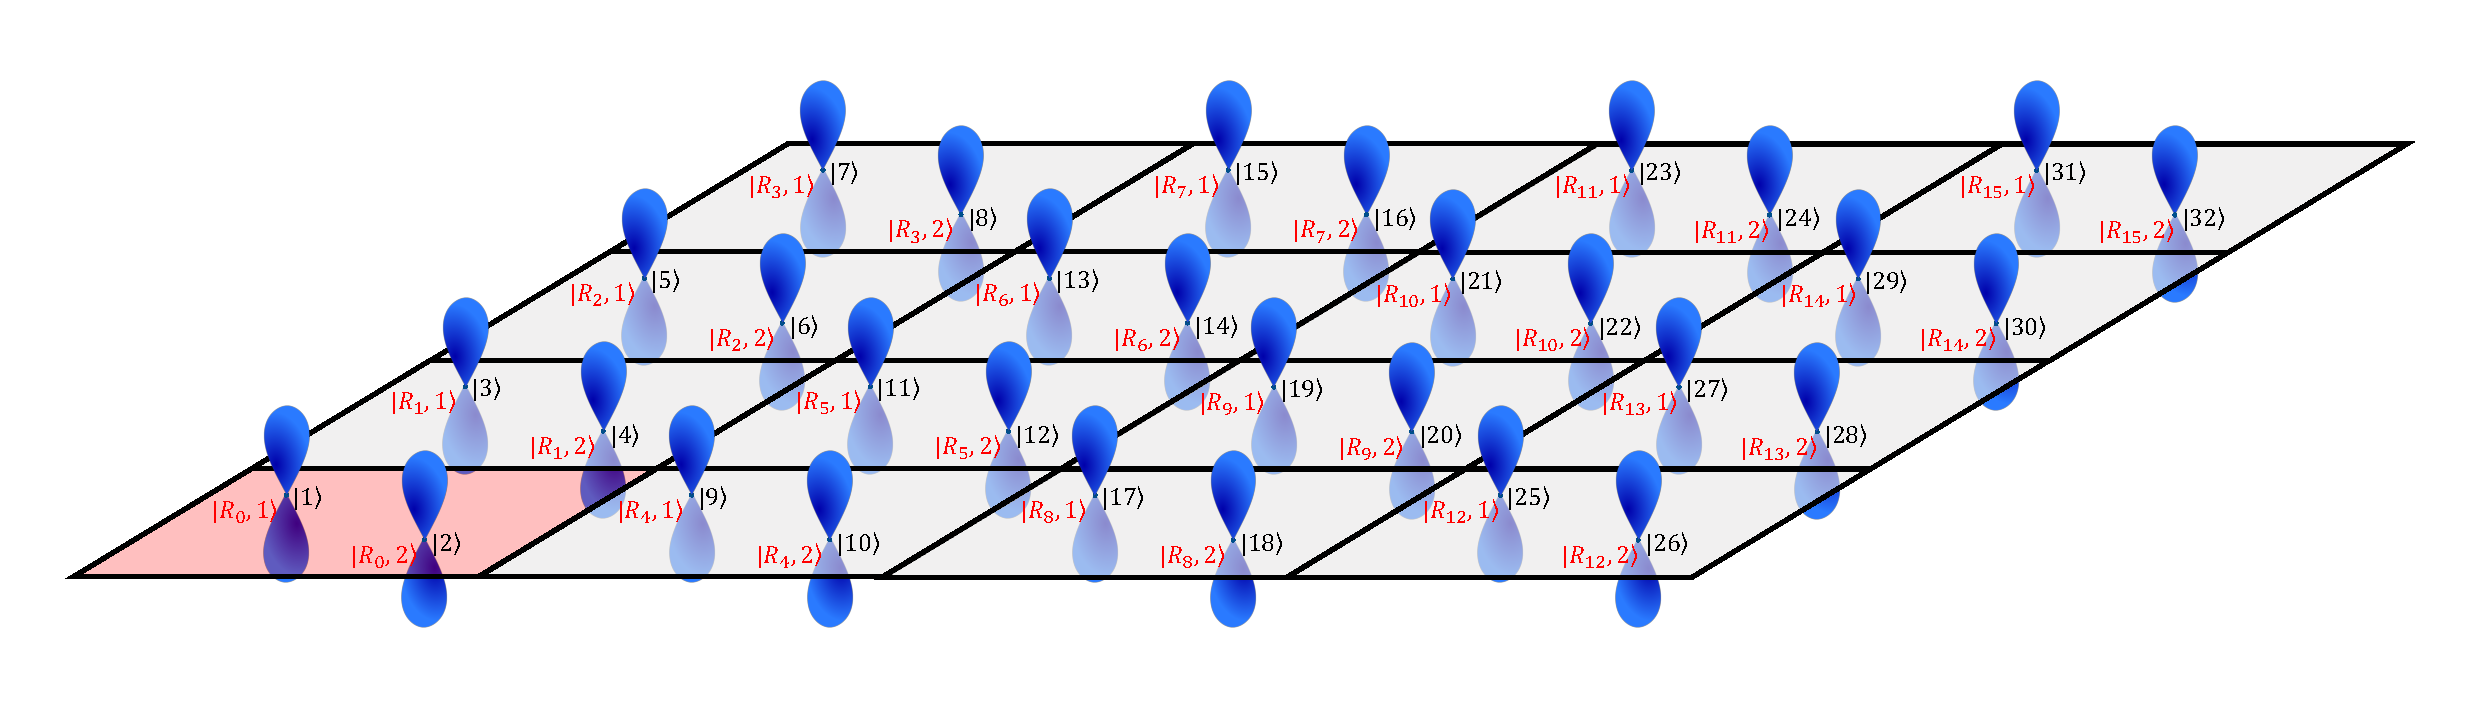
\includegraphics[width=\linewidth]{WF-pcell-scell.pdf}
    \caption[Schematic representation of the map connecting PC's and SC's Wannier functions]{Schematic representation of a two-dimensional 2-band model showing the connection between the PC and SC Wannier representations. In the primitive picture with a $4\times 4$ sampling of the BZ, the WFs are identified with the pair of labels $\{ n,\bR \}$ (red labels): the cell index $\bR$ taking four values and the band index $n$ taking two values. In the $4\times 4$ SC with $\Gamma$-sampling of the BZ, the eight WFs are labeled by only one quantum number (black labels), i.e.\ the SC band index $\alpha$ running over the eight states.}
    \label{fig:map-wf}
\end{figure}

In order to recover this band structure, several methods have been developed \cite{boykin_practical_2005, lee_band_2005, ku_unfolding_2010, popescu_extracting_2012, huang_general_2014, medeiros_effects_2014, zheng_quantum_2015}; our approach follows the same strategy of \cite{lee_band_2005} and exploits the Wannier nature of the variational orbitals. By means of the transformation linking WFs and BFs [see \cref{eq:wannier-function}], the matrix elements of the $\bk$-space Hamiltonian are obtained from those given by the Wannier-like variational orbitals via a (double) Fourier transform:
%
\begin{equation}
    \begin{split}
        h^{\rm KC}_{mn}(\bk,\bk') &= \sum_{\bR,\bR'} e^{-i\bk \cdot \bR} e^{i\bk' \cdot \bR'} \braket{w_{m\bR} | \hat{h}^{\rm KC}_{n\bR'} | w_{n\bR'}} \\
        &= \sum_{\bR,\bR'} e^{-i\bk \cdot \bR} e^{i\bk' \cdot \bR'} h^{\rm KC}_{mn}(\bR,\bR') ,
    \end{split}
    \label{eq:double-k-ham}
\end{equation}
%
where we introduced the matrix elements $h^{\rm KC}_{mn}(\bR,\bR') = \braket{w_{m\bR} | \hat{h}^{\rm KC}_{n\bR'} | w_{n\bR'}}$. If the Koopmans Hamiltonian is compliant with the translation symmetries of the system, the matrix elements satisfy the property
%
\begin{equation}
    \begin{split}
        h^{\rm KC}_{mn}(\bR,\bR') &= \braket{w_{m\bR} | \hat{h}^{\rm KC}_{n\bR'} | w_{n\bR'}} \\
        &= \braket{w_{m{\bm 0}} | \hat{h}^{\rm KC}_{n\bR'-\bR} | w_{n\bR'-\bR}} \\
        &= h^{\rm KC}_{mn}({\bm 0},\bR'-\bR) \equiv h^{\rm KC}_{mn}(\bR'-\bR) ,
    \end{split}
    \label{eq:trans-prop-koopmans-matrix-elements}
\end{equation}
%
that, if used in \cref{eq:double-k-ham}, yields a block-diagonal matrix (as expected from Bloch's theorem)
%
\begin{equation}
    h^{\rm KC}_{mn}(\bk,\bk') = h^{\rm KC}_{mn}(\bk) \delta(\bk - \bk')
    \label{eq:block-diagonal-koopmans-ham}
\end{equation}
%
with
%
\begin{equation}
    h^{\rm KC}_{mn}(\bk) = \sum_{\bR} e^{i \bk \cdot \bR} \braket{w_{m\bm{0}} | \hat{h}^{\rm KC}_{n\bR} | w_{n\bR}} = \sum_{\bR} e^{i \bk \cdot \bR} h^{\rm KC}_{mn}(\bR) ,
    \label{eq:hk-unfold}
\end{equation}
%
The diagonalization of the Hamiltonian with matrix elements defined by \cref{eq:hk-unfold}, yields the quasiparticle energies $\varepsilon_{n\bk}$ at any $\bk$-point.

In the SC approach the Brillouin zone reduces to a single point; as a consequence, the SC Hamiltonian in the Wannier representation loses the information about the lattice vectors $\{\bR\}$ and its matrix elements are labeled by the SC index only. In order to reconstruct the $\bk$-space Hamiltonian of \cref{eq:hk-unfold}, one must reconstruct the composite index $\{n,\bR\}$ of each WF from its supercell-picture index ${\alpha}$ (see \cref{fig:map-wf}). An effective way to do this is to first choose a reference PC and define the orbitals with the centers inside it as the ``$\bR=\bm{0}$ Wannier functions''. The second step consists of comparing all the other WFs in the supercell with those in the reference cell. If the Wannier translation property holds, we are able to connect each WF to its reference function $w_{\bm{0} n}$ and lattice vector $\bR$, defined as the distance between the centers of the two functions. If the system has more functions sharing the same center, one can look at the second-order moments ($\braket{x^2}$, $\braket{y^2}$, $\braket{z^2}$) to have a more detailed signature of WFs and, if needed, can move towards higher-order spatial moments until the character of each Wannier function is unequivocally defined \cite{shelley_automated_2011}.

As argued in Ref.~\cite{lee_band_2005}, \cref{eq:hk-unfold} not only applies to the points belonging to the $\bk$-mesh commensurate with the chosen supercell, but it is also an excellent interpolator. So, in order to calculate the band structure along any path in the Brillouin zone, we obtain the matrix elements of the $\bk$-space Hamiltonian by simply applying \cref{eq:hk-unfold} to any arbitrary $\bk$-point. In doing so, two approximations are applied to the matrix elements. To highlight such approximations -- and, especially, justify the fact that they have a negligible effect -- let us consider a point $\bk'$ which does not belong to the original sampling $\{ \bk \}$ of the BZ. In \cref{eq:hk-unfold}, the $\bk$-points must be commensurate\footnote{
A regular sampling of the BZ, made of $N_1 \times N_2 \times N_3$ $\bk$-points generates a system consisting of $N_1 \times N_2 \times N_3$ repetitions of the unit cell, each of which is identified by a lattice vector $\bR$; a set $\{ \bk \}$ which samples (regularly) the BZ is said to be commensurate to $\{ \bR \}$ (and viceversa) if the latter is the direct lattice with PBC set by $\{ \bk \}$.
}
with the set of lattice vectors $\{ \bR \}$ over which the sum runs, therefore, in order to compute the matrix elements $h^{\rm KC}_{mn}(\bk')$ we should, in principle, sum over a set $\{ \bR' \}$ which is commensurate to a sampling of the BZ that includes the point $\bk'$. When interpolating the matrix elements of the $\bk$-space Hamiltonian, we apply then a zero-padding technique \cite{buongiorno_nardelli_paoflow_2018}, where the contributions coming from the bigger lattice $\{ \bR' \}$ are neglected:
%
\begin{equation}
    \begin{split}
        h^{\rm KC}_{mn}(\bk') &= \sum_{\bR'} e^{i \bk' \cdot \bR'} \braket{w_{m\bm{0}} | \hat{h}^{\rm KC}_{n\bR'} | w_{n\bR'}}_{V'} \\
        &= \sum_{\bR} e^{i \bk \cdot \bR} \braket{w_{m\bm{0}} | \hat{h}^{\rm KC}_{n\bR} | w_{n\bR}}_{V'} + \sum_{\bR' \neq \bR} e^{i \bk \cdot \bR'} \braket{w_{m\bm{0}} | \hat{h}^{\rm KC}_{n\bR'} | w_{n\bR'}}_{V'} \\
        &\approx \sum_{\bR} e^{i \bk \cdot \bR} \braket{w_{m\bm{0}} | \hat{h}^{\rm KC}_{n\bR} | w_{n\bR}}_{V}
    \end{split}
    \label{eq:hk-interpolated}
\end{equation}
%
where $V$ and $V'$ are the volumes of the lattices $\{ \bR \}$ and $\{ \bR' \}$. In the last step the terms corresponding to lattice vectors not belonging to the original lattice -- i.e. $\bR' \neq \bR$ -- are neglected, and the integral to evaluate the matrix elements $h^{\rm KC}_{mn}(\bR)$ is calculated over the volume $V$ (rather than $V'$). The accuracy of the approximation is higher the smaller the contribution from these terms, i.e. the more localized the variational orbitals are, or the larger the supercell becomes. A poorly interpolated band structure is usually symptom of a significant contribution from the matrix elements corresponding to larger $\bR$-vectors, or of a non-negligible integral coming from the region $V' \setminus V$ in the calculation of the matrix elements $h^{\rm KC}_{mn}(\bR)$. Ultimately, the effects of such approximations are reduced by increasing the size of the supercell.

\subsubsection*{Smooth interpolation method}
As a consequence of what was just discussed, when reconstructing the band structure from a supercell calculation, one faces a trade-off: on one hand, a sufficiently large SC must be used to minimize the errors associated with neglecting long-range matrix elements of the Hamiltonian. But on the other hand, increasing the size of the SC dramatically increases the computational costs. In this scenario, one can exploit the fact that the Koopmans potential is a small, slowly varying correction on top of the original DFT Hamiltonian. If one decomposes the right-hand side of \cref{eq:hk-unfold} in its DFT and KC components,
%
\begin{equation}
    h^{\rm KC}_{mn}(\bR) \longrightarrow h^{\rm DFT}_{mn}(\bR) + v^{\rm KC}_{mn}(\bR) ,
\end{equation}
%
it is reasonable to assume that the major source of error comes from the interpolation of $h^{\rm DFT}_{mn}(\bR)$. This allows to improve the interpolation of the band structure by rewriting \cref{eq:hk-unfold} as
%
\begin{equation}
    h^{\rm KC}_{mn}(\bk) = \sum_{\bR'} e^{i \bk \cdot \bR'} h^{\rm DFT}_{mn}(\bR') + \sum_{\bR} e^{i \bk \cdot \bR} v^{\rm KC}_{mn}(\bR)
    \label{eq:hk-smooth}
\end{equation}
%
where the set of vectors $\{ \bR' \}$ now corresponds to a much larger supercell or, equivalently, it comes from a calculation with a denser $\bk$-points grid. This represents a significant saving in computational costs because the Koopmans calculation can be then performed on smaller supercells than would otherwise be necessary.

In order to have a consistent representation between (a) the DFT Hamiltonian defined  on a very dense grid, and (b) the KC potential on a coarser grid, it is important to have the same set of WFs for the two calculations. As long as this is fulfilled, the Koopmans Hamiltonian can be factorized as shown in \cref{eq:hk-smooth} and the DFT part can be obtained starting from a $\bk$-points grid dense enough to reliably interpolate the band structure.

We stress that this method has the one goal of improving the interpolation of the band structure. The convergence of other results, such as total energies and eigenvalues on the $\bk$-points grid commensurate with the supercell, is typically achieved with relatively small supercells. The technique depicted above does not affect any of these quantities and only improves the results for the electronic eigenvalues at $\bk$-points not included in the original Monkhorst-Pack grid.

\subsection{Computational codes\label{sec:computational-codes}}
The workflow to perform a full calculation of Koopmans functionals is rather complex, and follows different steps, each of which requires several calculations. The computation of the screening parameters is the most time-consuming part for both the implementations, as it requires multiple constrained self-consistent SC calculations in the finite-differences approach, and DFPT calculations involving double loops over the plane waves and the $\bk$-points in the linear response approach. Recently, efforts have been made to increase the computational efficiency by defining new strategies for the calculation of the screening parameters: a machine-learning-based approach developed by Schubert \emph{et al.} \cite{schubert_ml_2022}, which exploits the correlation between the shape of the (variational) orbital densities and the corresponding $\alpha_i$, has showed very promising results and could represent a breakthrough for KC calculations.

While the workflow for finite systems is simpler, though very similar, to the one for solids, here we specify to the latter case. For both the approaches, the entire procedure consists of three main steps: (i) the initialization, consisting of a standard DFT calculation followed by a Wannierization of the KS states, in order to obtain MLWFs that are either used as a non-self-consistent guess for the variational orbitals or as initial guess for the energy minimization; (ii) the computation of the screening parameters; (iii) the final Koopmans calculation followed, in the SC approach, by the unfolding procedure described in \cref{sec:unfolding-method}. Many efforts have been put into the automatization of the Koopmans workflow, which is now fully handled by a Python package \cite{linscott_koopmans_2022}, based on the atomic simulation environment (ASE) \cite{larsen_atomic_2017}. Below, we describe in detail the various steps workflow for the two approaches, while a schematic representation is showed in \cref{fig:workflow}.

\subsubsection{\kcp code and the finite-differences workflow}
The finite-differences approach is based on the \kcp implementation of Koopmans functionals, where \kcp stands for Koopmans-CP. This name stems from the fact that the Koopmans code was originally implemented (for technical reasons) within an old version of the Car-Parrinello (CP) code of the \qe (QE) distribution \cite{giannozzi_quantum_2009,giannozzi_advanced_2017}, although no part related to the proper CP molecular dynamics technique is normally used. \kcp allows performing spin-polarized calculations with both the KI and KIPZ functionals; also, it contains a direct energy minimization algorithm -- this is based on the conjugate-gradient and steepest-descent techniques, coupled with an implementation of the Gram-Schmidt orthogonalization method -- which is used to determine self-consistently the variational orbitals of the system. Besides, the ODD character of the energy gradient makes the minimization procedure much heavier with respect to standard DFT codes in terms of computational time and memory, due to the need to compute and store all the different orbital-dependent potentials. \kcp is a $\Gamma$-only code, which means that all the calculations are performed using the SC method. This is actually convenient in Koopmans functionals, where large unit cells are needed to reach a sufficient orbitals' localization (see discussion in \cref{sec:localization}), and represents the only way to compute the screening parameters by means of the finite-differences method. 

A standard workflow for periodic systems using the finite-differences approach starts from a DFT calculation using the LDA or PBE functional, followed by a Wannierization of the KS states. The KS-DFT calculation is carried out with the plane-waves (PW) code of QE, whereas the Wannier functions minimizing the spread functional of \cref{eq:wannier-spread-functional} -- i.e. the MLWFs -- are obtained from the Wannier90 code \cite{pizzi_wannier90_2020}. The computed WFs are then used to initialize the first Koopmans calculation using a set of trial screening parameters $\{ \alpha_i^{(0)} \}$, which are usually taken as the inverse of the dielectric constant (see \cref{sec:screening-parameters}). In the past, the initial KS-DFT calculation and the WFs were computed in an identical SC setup (same supercell and same energy cutoff) used then in \texttt{KCP}, in order to be consistent\footnote{
We remark that the philosophy of QE is that of expressing any wave function $\psi(\br)$ (as well as the other quantities of interest, such as the potentials, kinetic energy, etc.) as a linear combination of PWs, meaning that $\psi$ is described in terms of its Fourier components, $\{ \psi(\bG) \}$. Since the set of $\bG$-vectors is fully defined by the geometry of the cell and by the energy cutoff, the $\bG$-vectors, and so the Fourier components of $\psi$, are different between PC and SC.
}
with the input wave functions expected by the \kcp code. The problem with this strategy is that the resulting MLWFs would generally break the translation property \eqref{eq:trans-prop-wannier} with respect to the PC's lattice vectors. The $\Gamma$-only calculations reported in Ref.~\cite{nguyen_koopmans-compliant_2018} were not affected by this issue, whereas it became crucial in this work to find a way around it in order to recover the compliance with Bloch's theorem and be able to compute PC band structures. That was done by computing the MLWFs starting from a PC calculation with a sampling of the BZ commensurate to the SC used later on -- in this way the resulting WFs would satisfy \cref{eq:trans-prop-wannier} by construction -- and then unfolding such WFs from the PC to the SC. The procedure to extend the WFs from the PC to the SC was implemented within a private version of the QE \texttt{pw2wannier90} code.

\begin{figure}
    \centering
    \subfloat[]{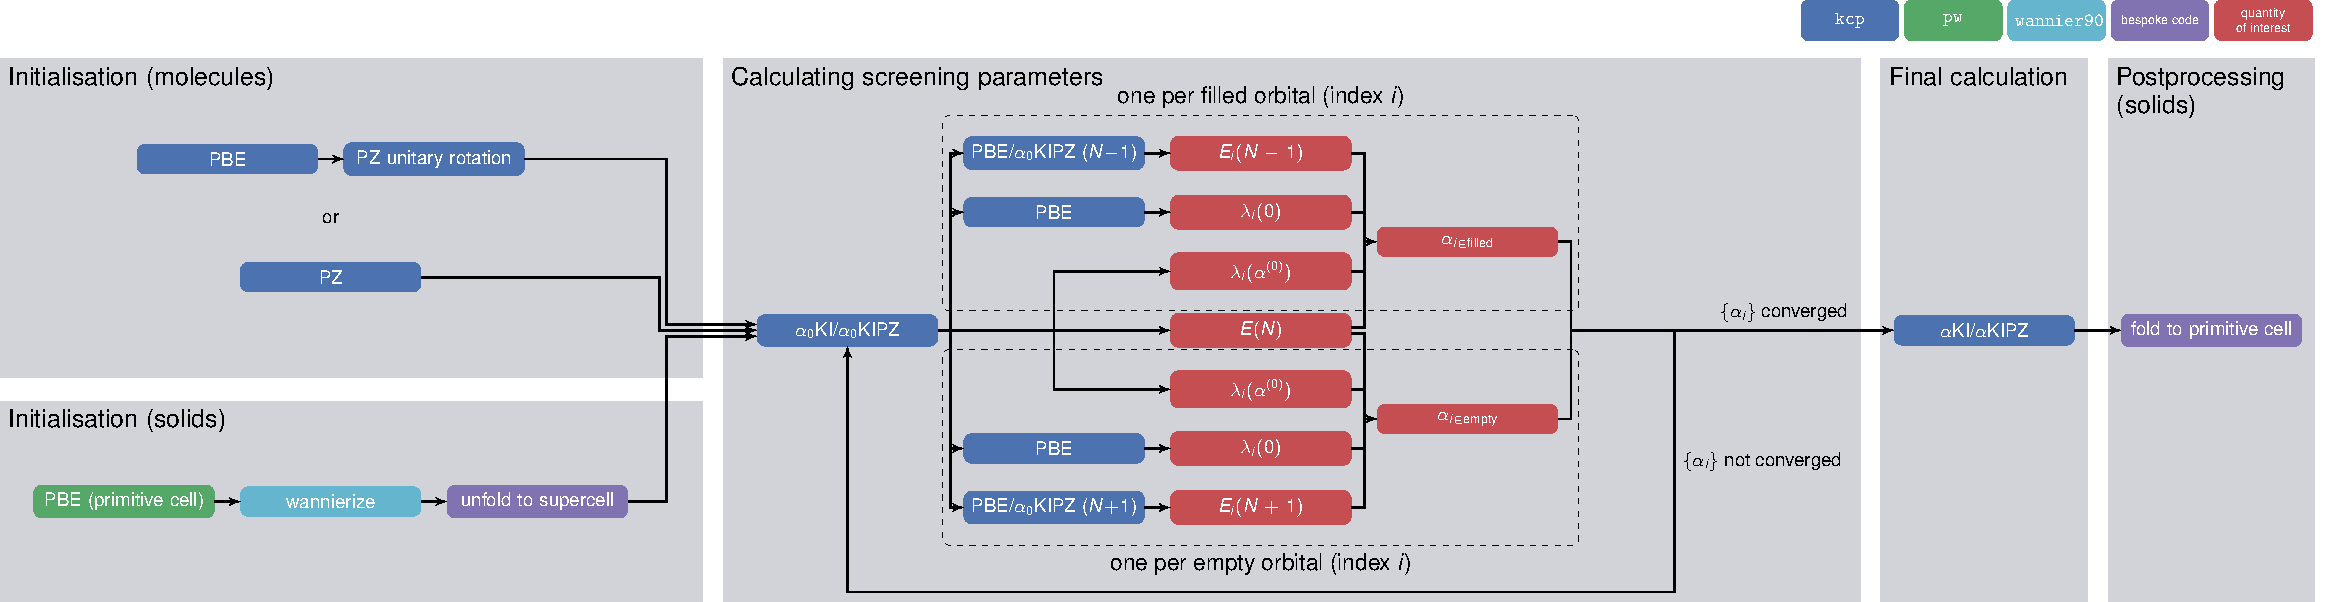
\includegraphics[width=\linewidth]{dscf_workflow.pdf}} \\
    \subfloat[]{\includegraphics[width=\linewidth]{dfpt_workflow.pdf}}
    \caption[Finite-differences and DFPT workflow schemes]{Schematic representation of the workflows for the (a) SC-based finite-differences approach and the (b) PC-based linear response approach, using PBE as base DFT functional.}
    \label{fig:workflow}
\end{figure}

Once the initialization step is concluded, two different directions can be taken: a non-self-consistent road, where the computed MLWFs are taken as variational orbitals with no further optimization, or a self-consistent road, where the MLWFs are the starting point for the energy minimization which brings to the actual self-consistent variational orbitals. For KI calculations, where the ground-state density is the same of the underlying DFT functional -- this corresponds also to the density given by the computed WFs -- the default strategy is represented by the first option (followed also in this thesis); alternatively, given the interpretation of the KI functional as a KIPZ functional with a vanishingly small PZ term (see paragraph at the end of \cref{sec:variational-procedure}), the self-consistent variational orbitals can be obtained via an inner loop only minimization of the energy functional (no outer loop since we do not need to update the total density). For KIPZ calculations, since also the ground-state density changes, the variational orbitals are normally computed self-consistently via a combined outer-inner loop minimization. In this thesis we often report results obtained from a \emph{perturbative KIPZ} (pKIPZ) approach: essentially, this consists of a KIPZ calculation where the variational orbitals, as well as the screening parameters, are taken from a prior KI calculation.

After the variational orbitals have been obtained, the orbital-dependent screening parameters are computed. As discussed in \cref{sec:screening-parameters}, these are obtained performing constrained self-consistent calculations where the selected orbital is each time kept frozen, and its occupation is set to zero (for occupied states) or to one (for empty states). This allows to calculate the energy difference $\Delta E^{\rm KC}_i$ appearing in \cref{eq:screening-parameter-dscf} which, together with the expectation values of the DFT and Koopmans Hamiltonians over the frozen orbital, represent all the ingredients needed to compute $\alpha_i$. We point out that in this phase, finite-size corrections are introduced in order to account for the spurious interactions between the periodic replicas of the introduced electric charge. Details about this aspect are given in \cref{sec:makov-payne}.

Finally, we perform a conclusive Koopmans calculation with the computed screening parameters. The resulting Hamiltonian is then unfolded to the PC and interpolated along a chosen path in the BZ; its eigenvalues provide the band structure of the system.

\subsubsection{\kcw code and the DFPT workflow}
The \kcw code (standing for Koopmans-Compliant Wannier method) contains a primitive cell implementation of Koopmans functionals (only for the KI functional, for the moment), where the screening parameters are computed from DFPT for a second-order approximation of the Koopmans correction terms \cite{colonna_koopmans_2022}. As for the standard KI workflow in the finite-differences approach, MLWFs are taken as a guess for the variational orbitals. The workflow then is pretty much the same of the one depicted for the finite-differences approach, with the only \emph{caveat} of the different method for the computation of $\{ \alpha_i \}$. Also, the absence of a ``PC to SC transition'' prevents the need for an unfolding technique to extend the WFs to the SC first, and to unfold the Koopmans Hamiltonian back to the PC after.

Since the release of the version 7.1 of QE (June 2022), \kcw is officially part of the QE package suite. On the other hand, \kcp, as well as the Python package handling the workflows, are part of a private repository which will be soon released \cite{linscott_koopmans_2022}.

\subsection{Finite-size corrections\label{sec:makov-payne}}
In periodic boundary conditions, calculations performed on charged systems require accounting for the spurious interactions between the introduced electric charge and its periodic replicas. Given the slow decay of the Coulomb potential, the size of the cell required to kill such self-interactions is usually impracticable -- even though, for quasi-metallic systems the dielectric screening of the material often damps sufficiently the electrostatic potential generated by a localized charge -- and demands for a different treatment of these finite-size effects. Several methods have been developed in the past years to tackle this problem \cite{gygi_self-consistent_1986,martyna_reciprocal_1999,dabo_electrostatics_2008,freysoldt_fully_2009,komsa_finite-size_2012}; here we followed the strategy proposed by Makov and Payne (MP), who computed the electrostatic energy of a point charge in a cubic system \cite{makov_periodic_1995}:
%
\begin{equation}
    E = E^{\rm pbc}(L) + \frac{q^2 \alpha}{2L} + \frac{2\pi q Q}{3L^3} + \mathcal{O}(L^{-5}) ,
    \label{eq:makov-payne-corrections}
\end{equation}
%
where $E^{\rm pbc}$, is the electrostatic energy of the point-charge in periodic boundary conditions embodying the interaction with the replicas, $L$ is the side of the cubic cell, $q$ is the charge, and $Q$ is the quadrupole moment -- if the introduced charge has a density $\rho_{\rm c}(\br)$, the quadrupole is defined as $Q = \int d\br \rho_{\rm c}(\br)r^2$. In this context $\alpha$ represents the Madelung constant which is given for any cubic lattice; here, $\alpha$ is calculated during the Koopmans workflow via a technique resembling the Ewald summation, which allows to compute a MP-like first-order correction also for non-cubic systems. In a dielectric medium, the natural extension of \cref{eq:makov-payne-corrections} includes the dielectric constant and reads as
%
\begin{equation}
    E = E^{\rm pbc}(L) + \frac{q^2 \alpha}{2\epsilon L} + \frac{2\pi q Q}{3\epsilon L^3} + \mathcal{O}(L^{-5}) .
    \label{eq:makov-payne-corrections-dielectric}
\end{equation}

Within the Koopmans workflow, the only part of the calculation that involves a system with a net charge is during the computation of the screening parameters, by means of the finite-differences method. The energy differences obtained by emptying (filling) an occupied (empty) variational orbital are then corrected \emph{a posteriori} in the following way:
%
\begin{equation}
    \begin{split}
        E(N) - E_i(N-1) \ &\longrightarrow \ E(N) - E_i(N-1) - \frac{q^2 \alpha}{2\epsilon L} \\
        E_i(N+1) - E(N) \ &\longrightarrow \ E_i(N+1) - E(N) + \frac{q^2 \alpha}{2\epsilon L} ,
    \end{split}
    \label{eq:dscf-corrected-makov-payne}
\end{equation}
%
where the quadrupole term of \cref{eq:makov-payne-corrections} has been excluded due to technical reasons (these are linked to the difficulty to compute the quadrupole moment for a generic variational orbital). When it was possible, the corrections of \cref{eq:dscf-corrected-makov-payne} were tested on the systems considered in this thesis. Few examples of convergence studies for the first-order MP corrections are showed in \cref{fig:convergence-makov-payne}: the corrected and uncorrected energy differences, resulting from the emptying of one of the occupied Wannier-like variational orbitals, were compared at increasing system's sizes for LiF, C, and Si. The difficulty of this study lies in the necessity of keeping the same Wannier function when passing from one SC to another, in order to have a meaningful comparison between the energies at different system's sizes. For LiF and C, we observe a consistency between the corrected and uncorrected extrapolated energies at infinite distances; as expected, the MP-corrected energies converge much more rapidly and justify the use of such corrections as long as the considered orbitals are sufficiently localized. On the other hand, for systems with a very small band gap like Si, the screening MP corrections poorly fail: this is not surprising, as in these situations the screening effects of the material become dominant, and the simple extension of the MP model via the insertion of the dielectric constant is not sufficient to account for the actual response of the material. On the bright side, for such systems, the screening of the material naturally damps the Coulomb potential, and the residual energy coming from the interaction between the periodic replicas is not very significant and can be neglected.

\begin{figure}
    \centering
    \subfloat[]{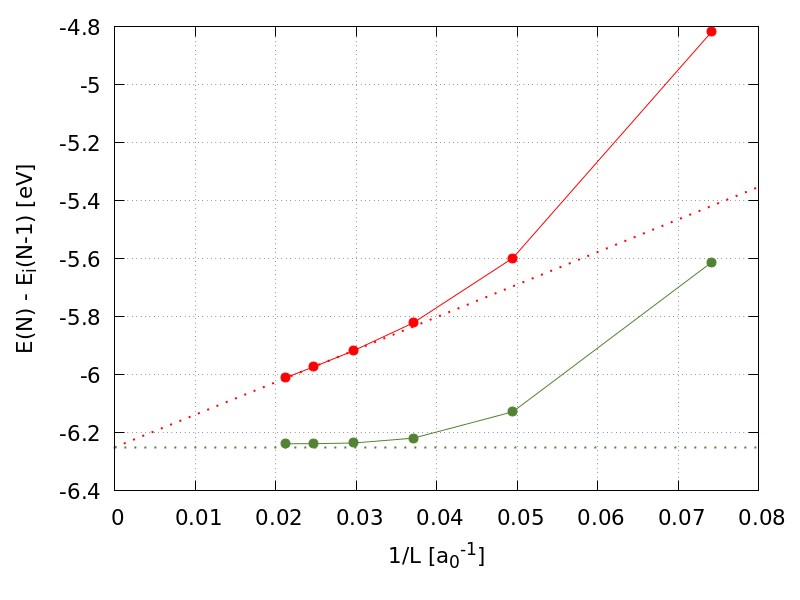
\includegraphics[width=0.5\linewidth]{c_mp.png}} 
    \subfloat[]{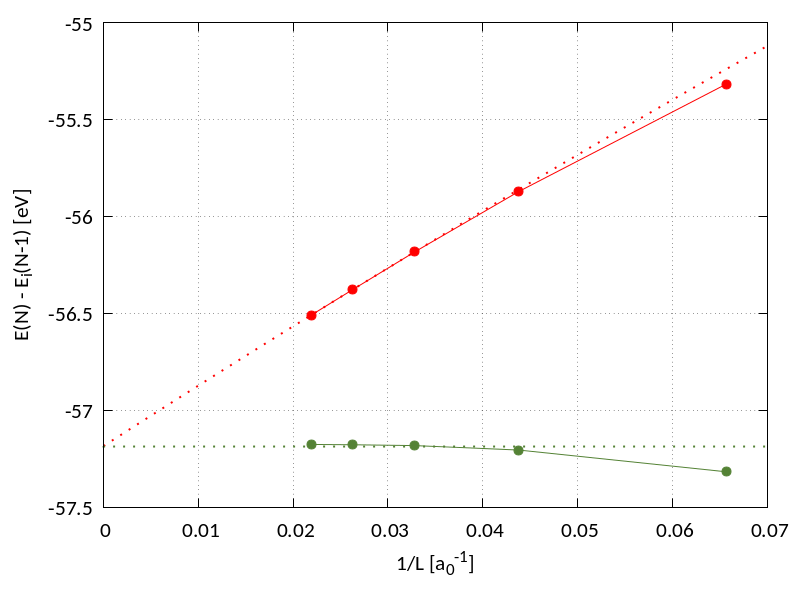
\includegraphics[width=0.5\linewidth]{lif_mp.png}} \\
    \subfloat[]{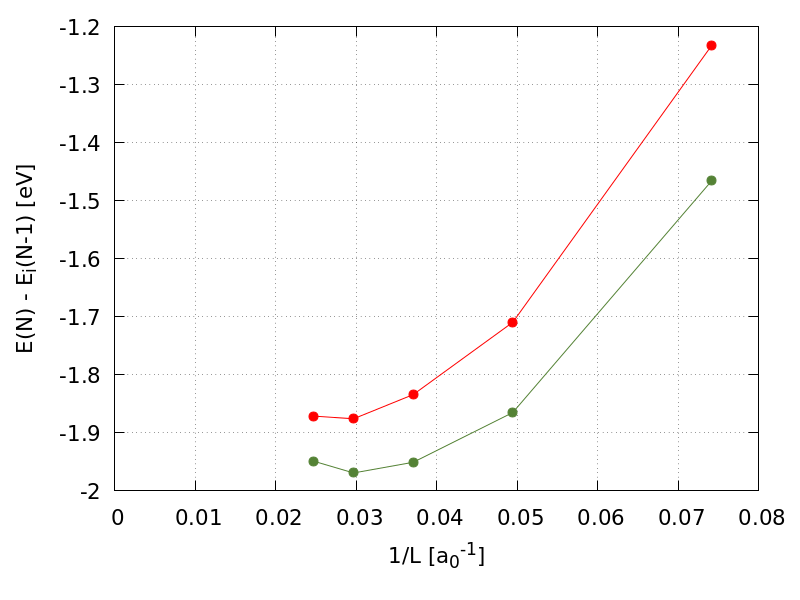
\includegraphics[width=0.5\linewidth]{si_mp.png}}
    \caption[Convergence finite-size corrections for the finite-differences method]{The bare (in red) and corrected (in green) [as in \cref{eq:makov-payne-corrections-dielectric}] energy differences are compared at different sizes for three prototypical systems: (a) a wide band gap insulator, i.e. lithium fluoride, (b) a medium band gap semiconductor, i.e. diamond, and (c) a small band gap material, i.e. silicon. The energies were computed at the PBE level, and for each system the orbitals frozen were taken from the valence band.}
    \label{fig:convergence-makov-payne}
\end{figure}

\section{Results and discussions\label{sec:results-bands}}
In this section we report the results obtained for a set of benchmark semiconductors and insulators using the two approaches described in the previous section. The base DFT functionals used in these calculations are PBE, for the finite-differences approach, and LDA, for the linear response approach. As for QE's implementation of DFT, we take advantage of the pseudopotential method to model the electron-ion interactions: more specifically, we used the optimized norm-conserving Vanderbilt pseudopotentials \cite{hamann_optimized_2013,hamann_erratum_2017} taken from the SG15 \cite{schlipf_optimization_2015} and DOJO \cite{van_setten_pseudodojo_2018} libraries. For the elemental compounds, the energy cutoffs have been chosen from the convergence studies provided by the standard solid state pseudopotentials precision protocol \cite{prandini_precision_2018}, while for the five binary compounds the cutoff was chosen by converging the KS-DFT band gap within 5~\mev. Unless specified otherwise, the employed $\bk$-point Monkhorst-Pack grids to sample the BZ (thus the sizes of the SCs used in the finite-differences approach) were $4\times 4\times 4$.

The band structure of Si, C, BN, Ge, GaAs, MgO, and LiF, computed with the finite-differences approach, are showed in \cref{sec:results-dscf}, whereas in \cref{sec:results-dfpt} we report the band structure of GaAs and ZnO as obtained from the linear response approach. All the materials have been modeled using their stable experimental structure under standard conditions of temperature and pressure: cubic rock-salt for MgO and LiF, hexagonal wurtzite for ZnO, and diamond (or zincblende) for all the rest. Experimental values for the lattice constants have been taken from Ref.~\cite{madelung_semiconductors_2004} or from the inorganic crystal structure database (ICSD) \cite{icsd_website}.

\subsection{Finite differences\label{sec:results-dscf}}

\begin{figure}
    \centering
    %
    \subfloat[Si: KI]{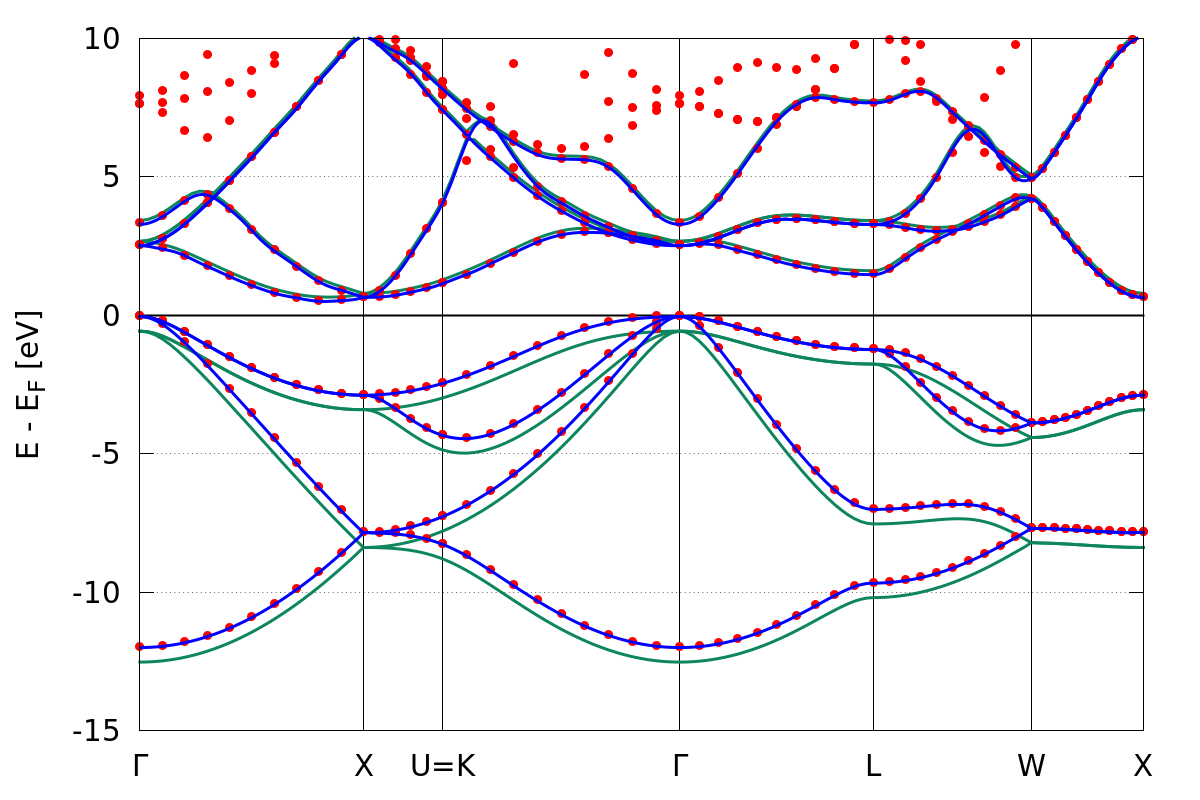
\includegraphics[width=0.5\linewidth]{Si_ki_bands.png}}
    \subfloat[Si: KIPZ]{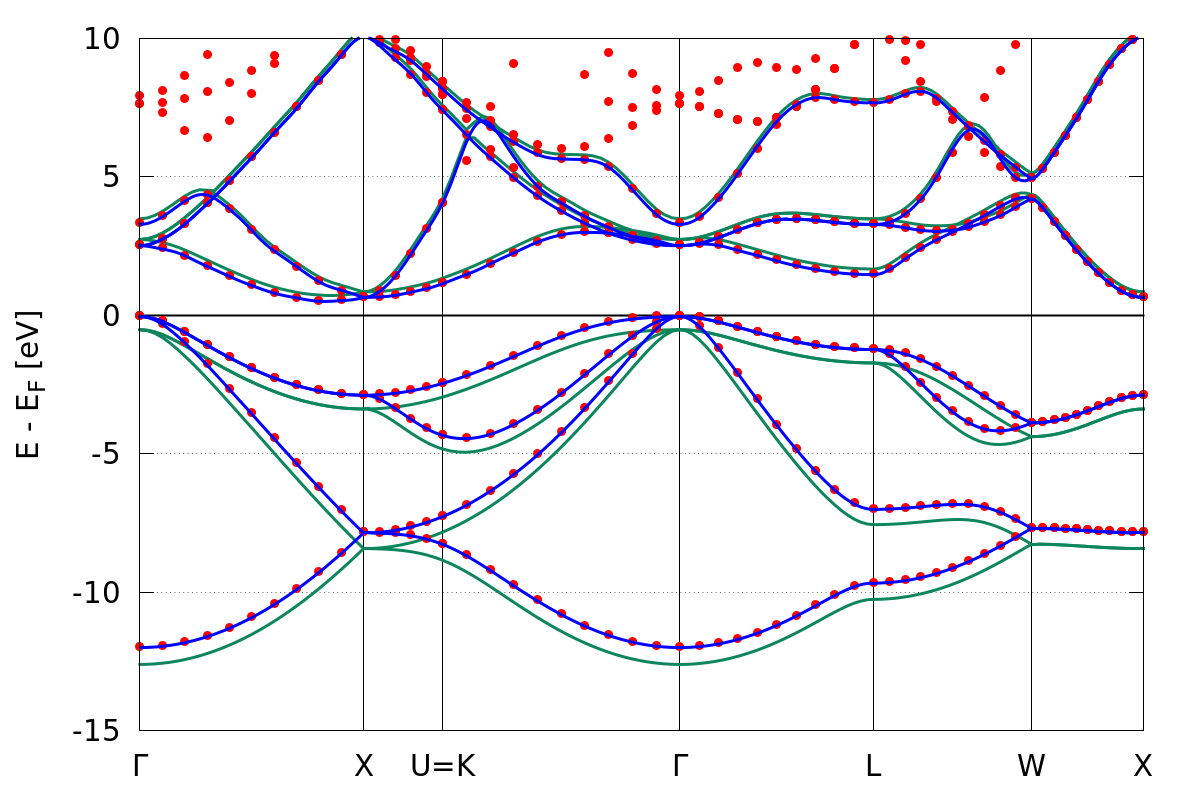
\includegraphics[width=0.5\linewidth]{Si_kipz_bands.png}} \\
    \subfloat[C: KI]{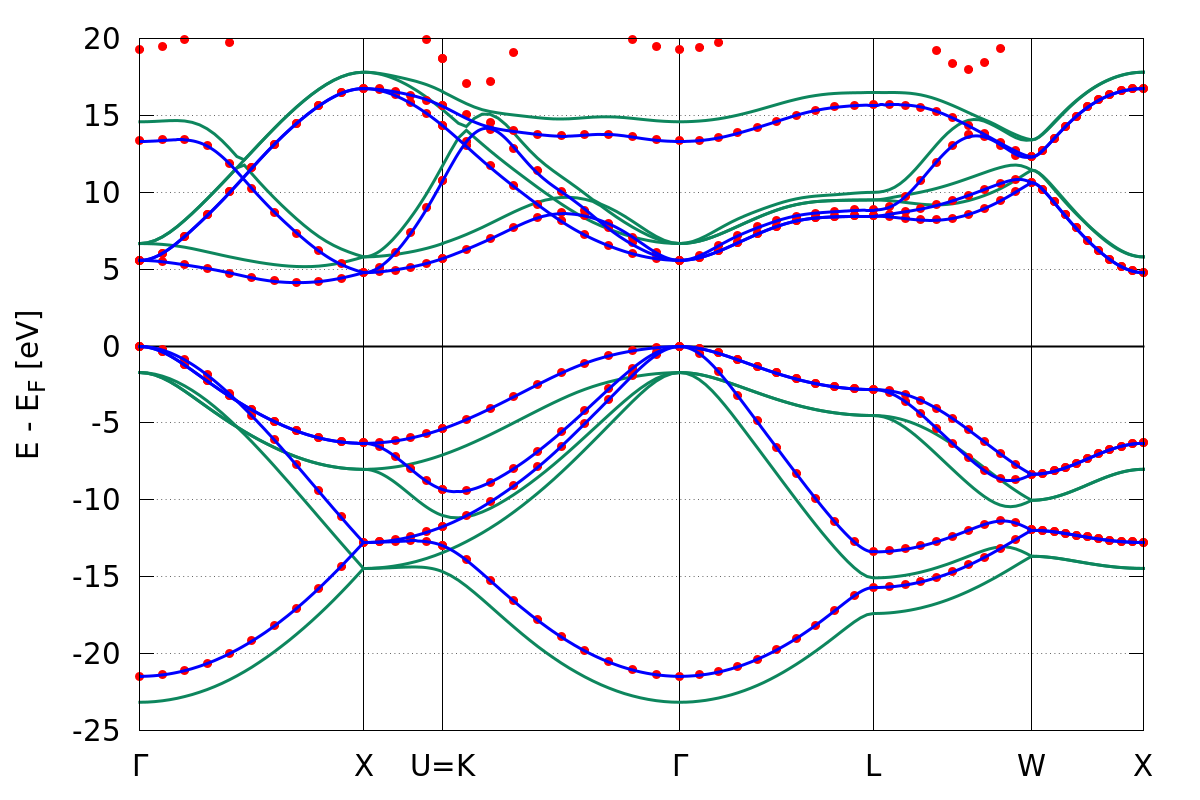
\includegraphics[width=0.5\linewidth]{C_ki_bands.png}}
    \subfloat[C: KIPZ]{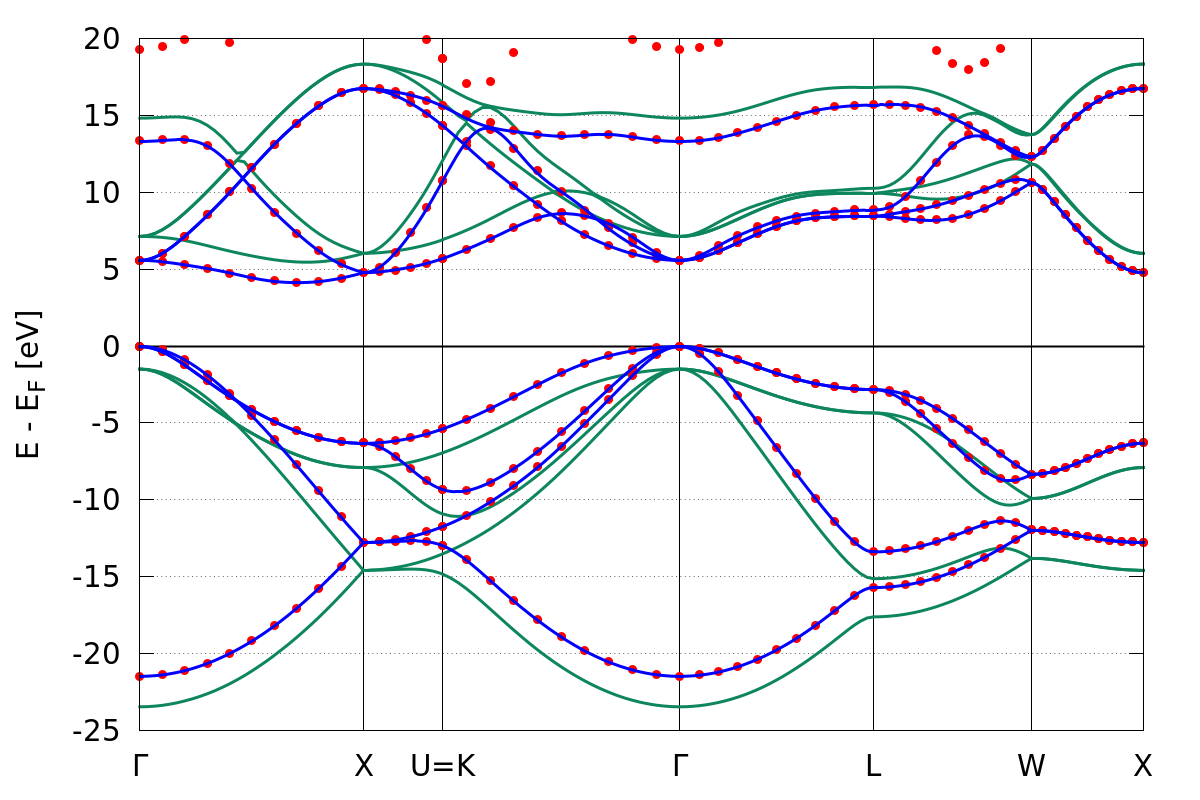
\includegraphics[width=0.5\linewidth]{C_kipz_bands.png}} \\
    \subfloat[BN: KI]{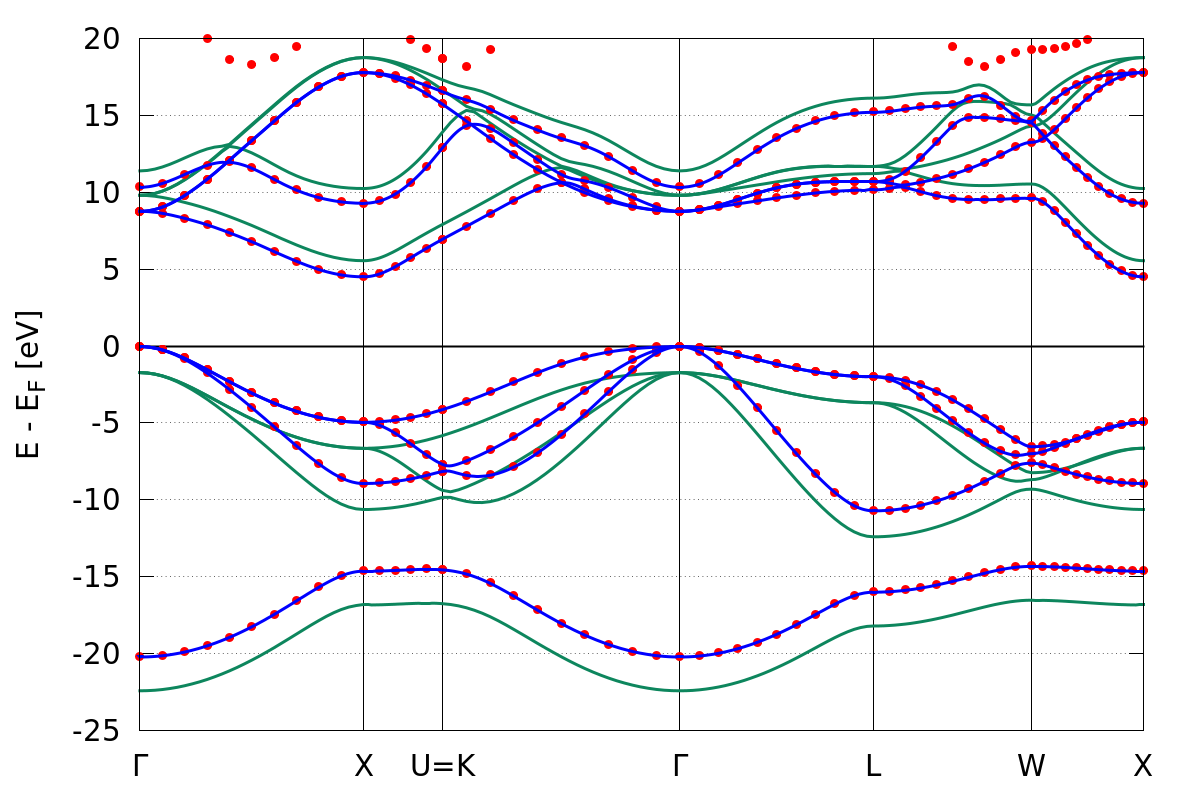
\includegraphics[width=0.5\linewidth]{BN_ki_bands.png}}
    \subfloat[BN: KIPZ]{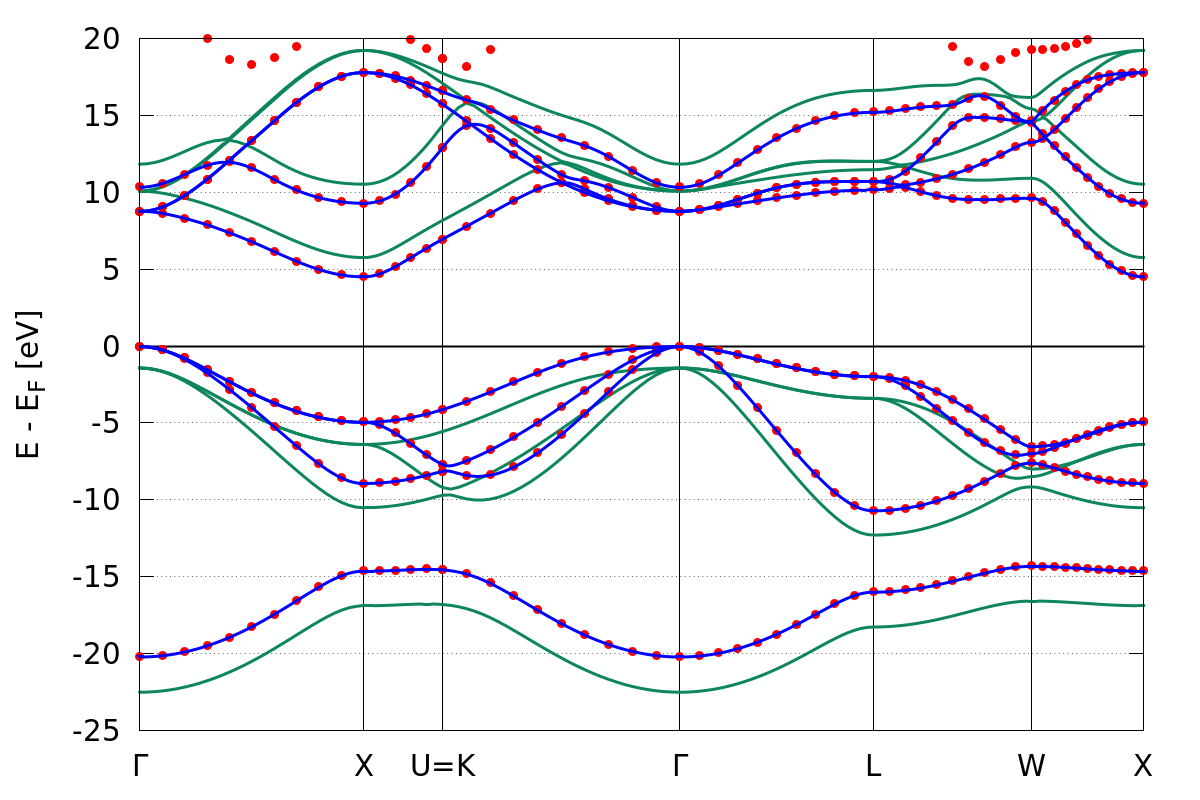
\includegraphics[width=0.5\linewidth]{BN_kipz_bands.png}}
    %
    \vspace{5mm}
    %
    \begin{tabularx}{\linewidth}{*{4}{>{\centering\arraybackslash}X}}
        \hline
        \hline
        & Si & C & BN \\
        \hline
        occupied & $sp^3$ & $sp^3$ & N: $s$, $p$ \\
        empty    & $sp^3$ & $sp^3$ & B: $s$, $p$ \\
        \hline
    \end{tabularx}
    %
    \caption[KI and KIPZ band structures of Si, C, and BN]{Band structure of Si, C, and BN: the red dots represent the PBE band structure calculated explicitly, while the blue lines are the interpolated PBE bands obtained with Wannier90; the green lines give the interpolated KI and KIPZ bands. The zero of the energy was set at the PBE Fermi level. At the bottom we report the initial atomic projectors for the Wannierization.}
    \label{fig:bands-1-si-c-bn}
\end{figure}

\begin{figure}
    \centering
    %
    \subfloat[Ge: KI]{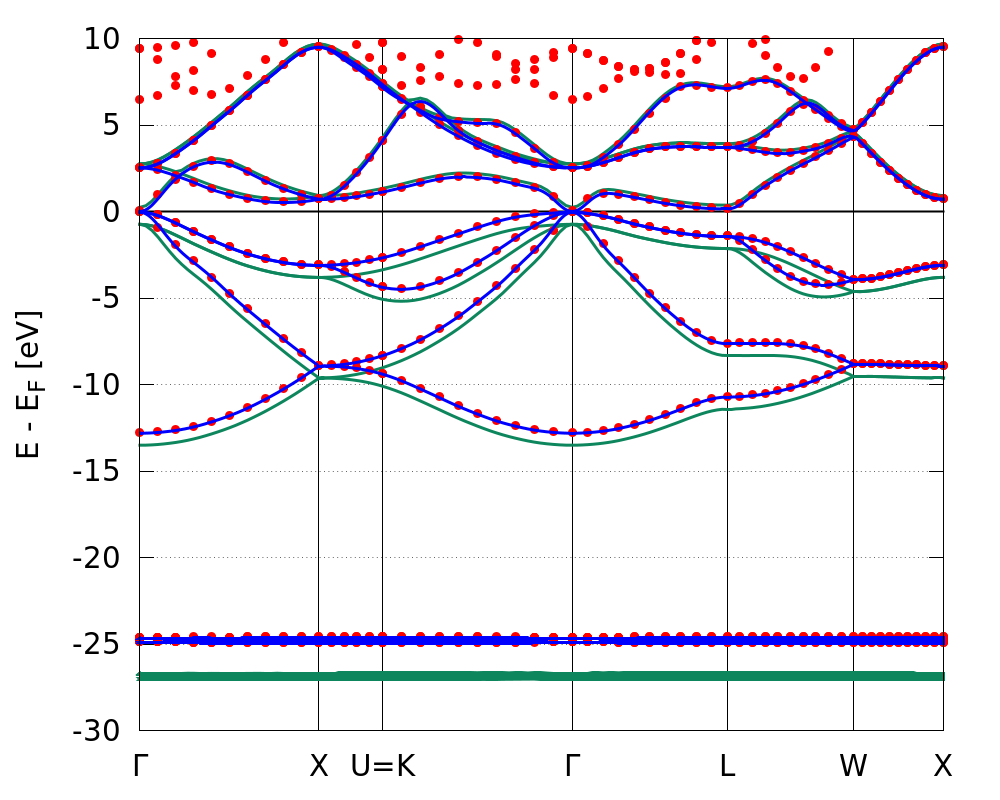
\includegraphics[width=0.5\linewidth]{Ge_ki_bands.png}}
    \subfloat[Ge: KIPZ]{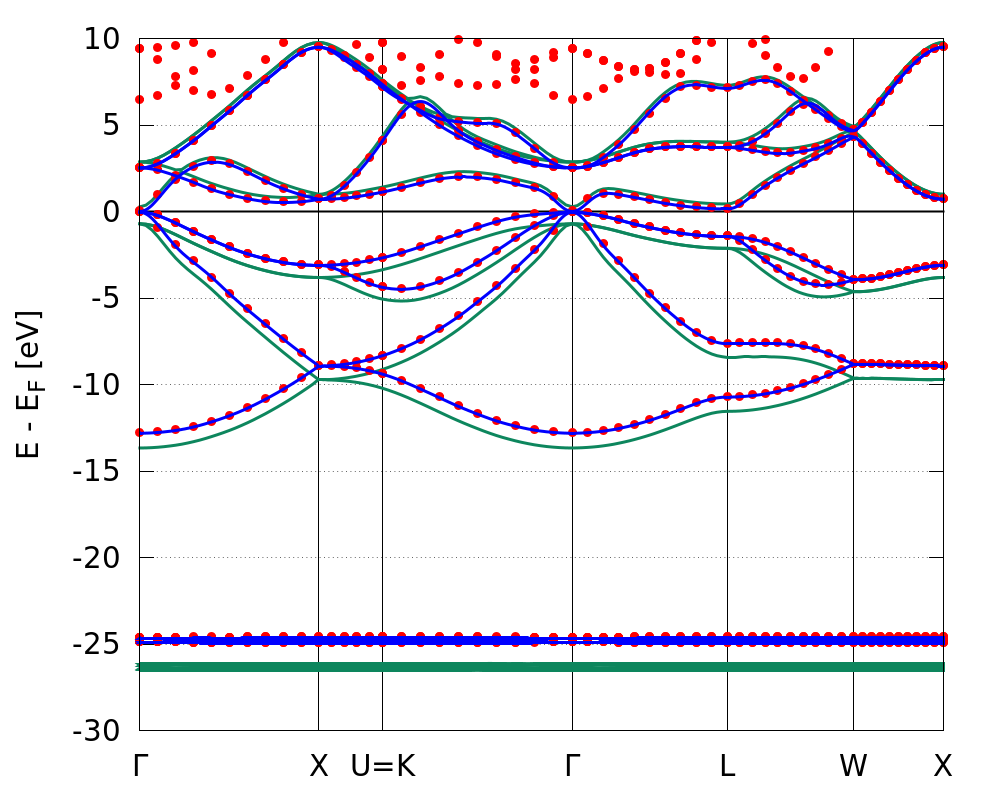
\includegraphics[width=0.5\linewidth]{Ge_kipz_bands.png}} \\
    \subfloat[GaAs: KI]{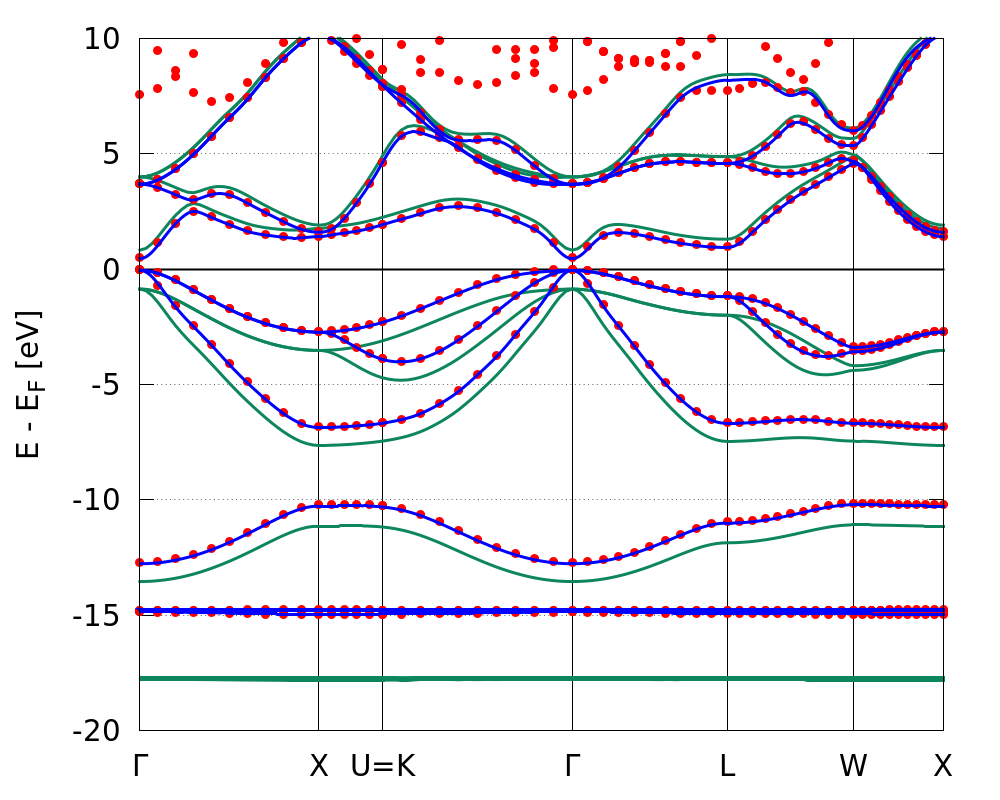
\includegraphics[width=0.5\linewidth]{GaAs_ki_bands.png}}
    \subfloat[GaAs: KIPZ]{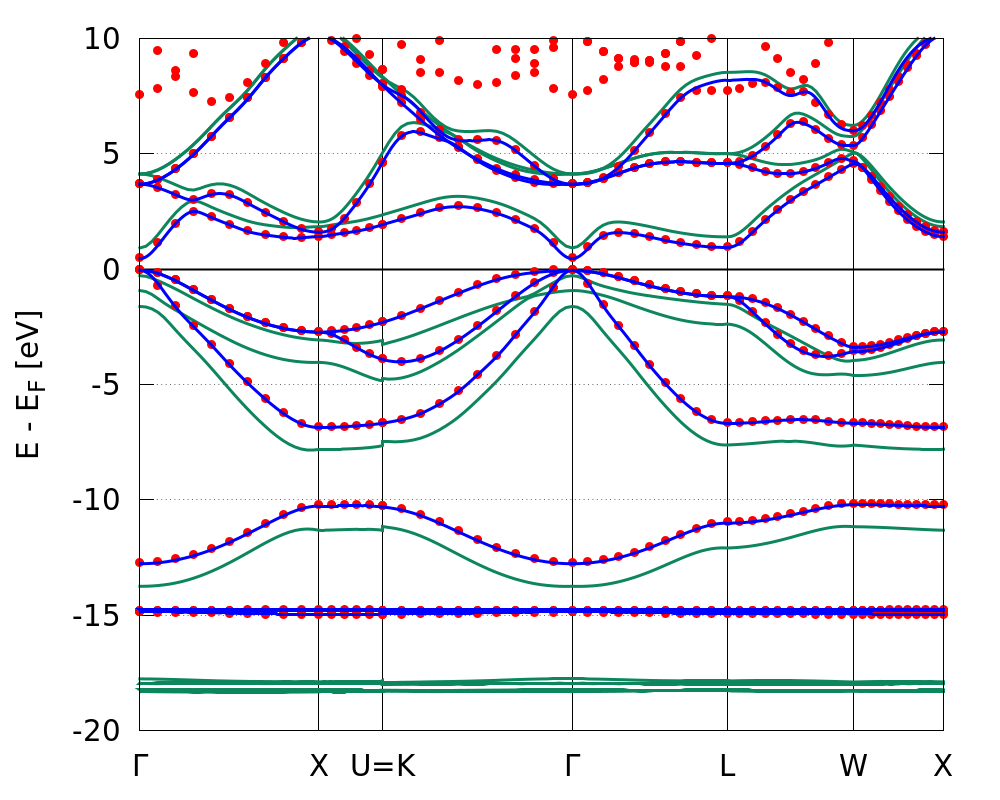
\includegraphics[width=0.5\linewidth]{GaAs_kipz_bands.png}}
    %
    \vspace{5mm}
    %
    \begin{tabularx}{\linewidth}{*{3}{>{\centering\arraybackslash}X}}
        \hline
        \hline
        & Ge & GaAs \\
        \hline
        occupied & $d$, $d$, $sp^3$ & $d$, $sp^3$ \\
        empty    & $sp^3$           & $sp^3$      \\
        \hline
    \end{tabularx}
    %
    \caption[KI and KIPZ band structures of Ge and GaAs]{As per \cref{fig:bands-1-si-c-bn}, here we show the band structures of Ge and GaAs obtained from the KI and KIPZ functionals.}
    \label{fig:bands-2-ge-gaas}
\end{figure}

\begin{figure}
    \centering
    %
    \subfloat[MgO: KI]{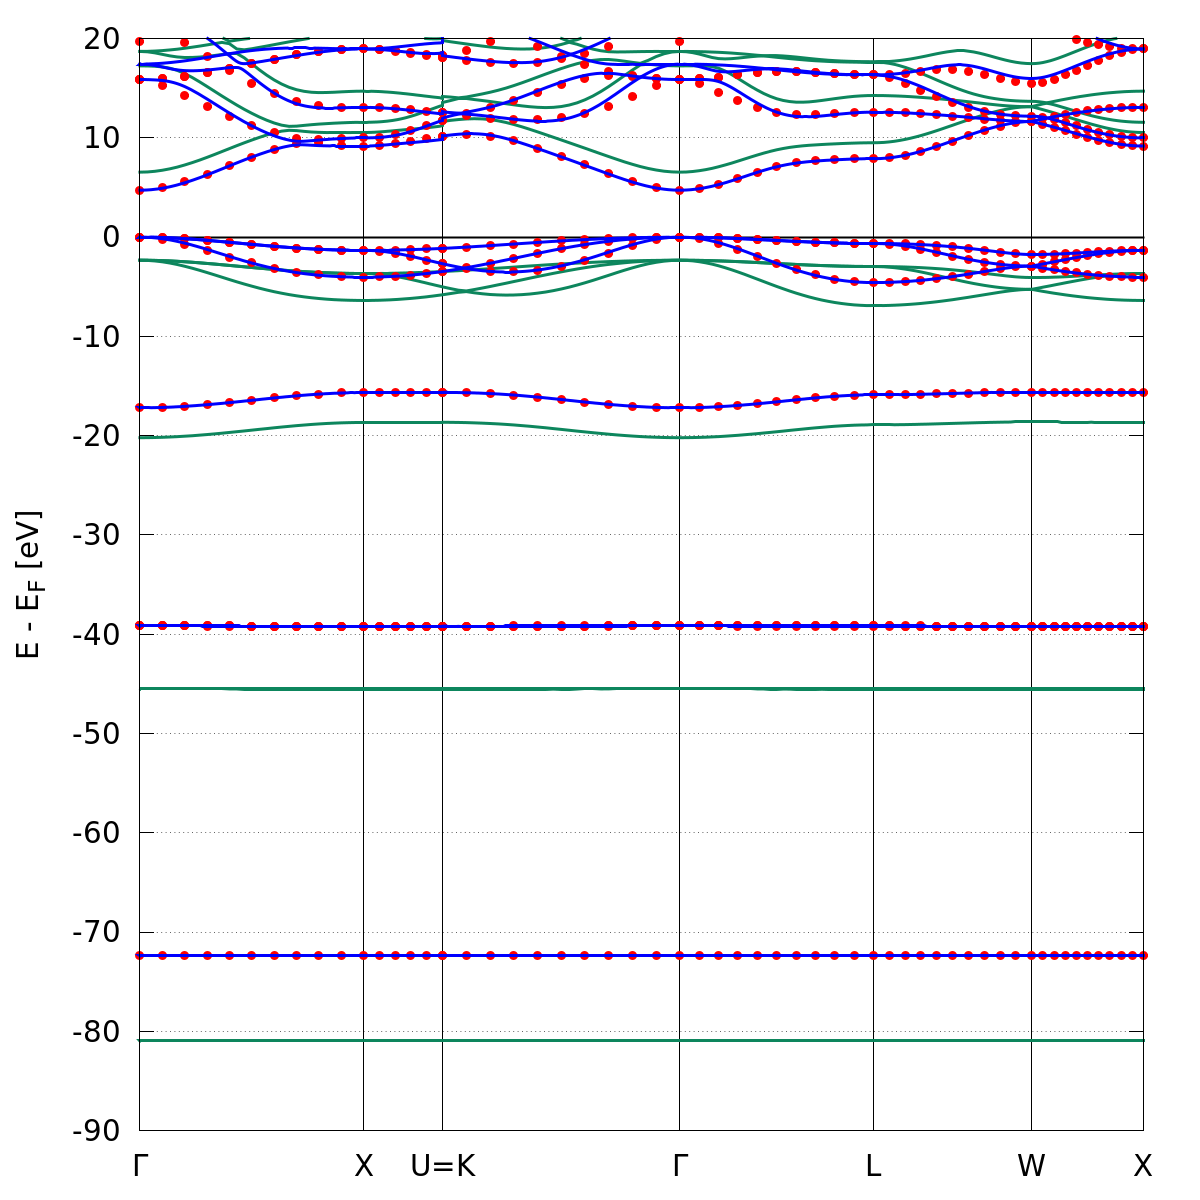
\includegraphics[width=0.5\linewidth]{MgO_ki_bands.png}}
    \subfloat[MgO: KIPZ]{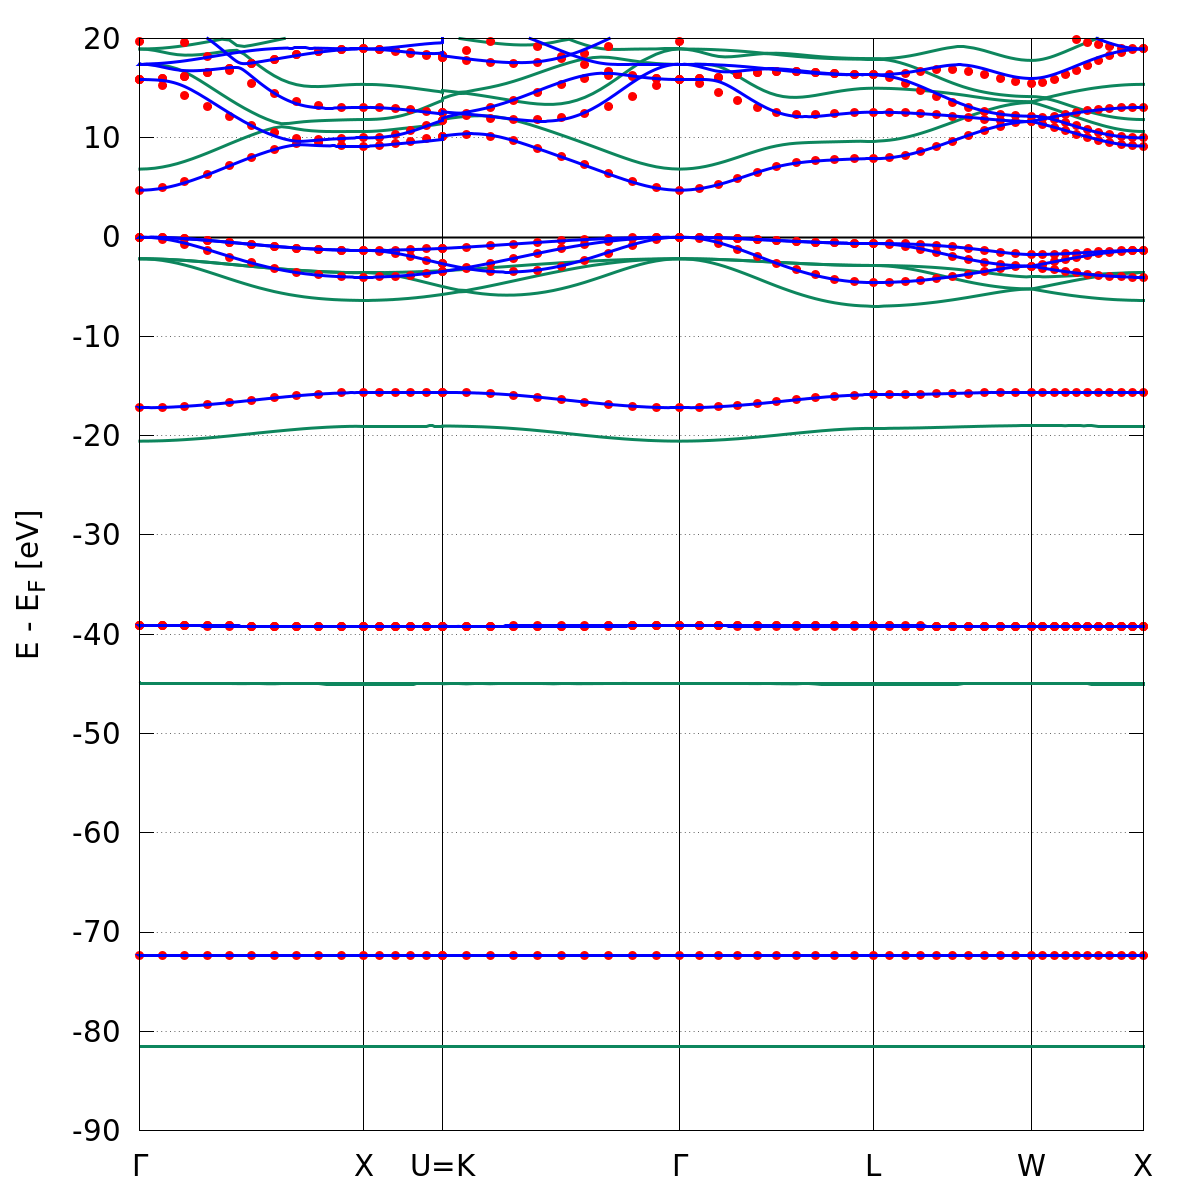
\includegraphics[width=0.5\linewidth]{MgO_kipz_bands.png}} \\
    \vspace{5mm}
    \subfloat[LiF: KI]{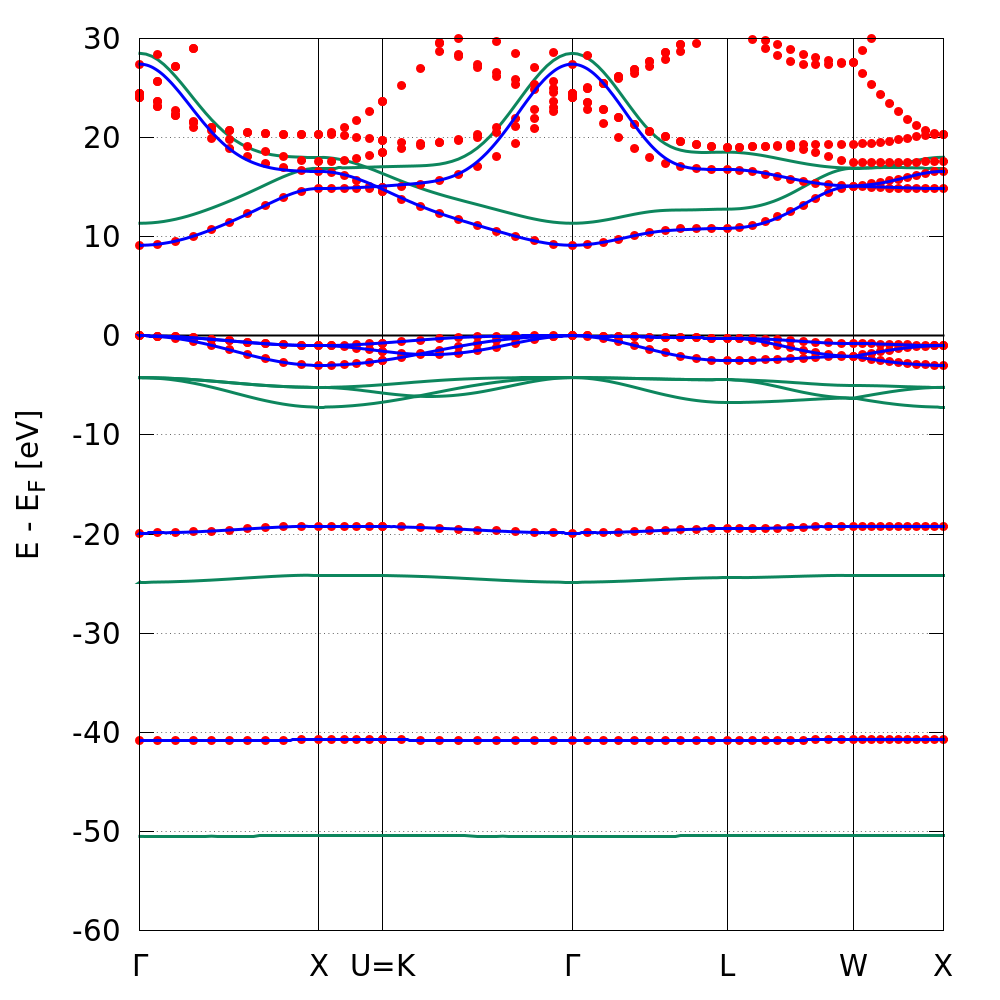
\includegraphics[width=0.5\linewidth]{LiF_ki_bands.png}}
    \subfloat[LiF: KIPZ]{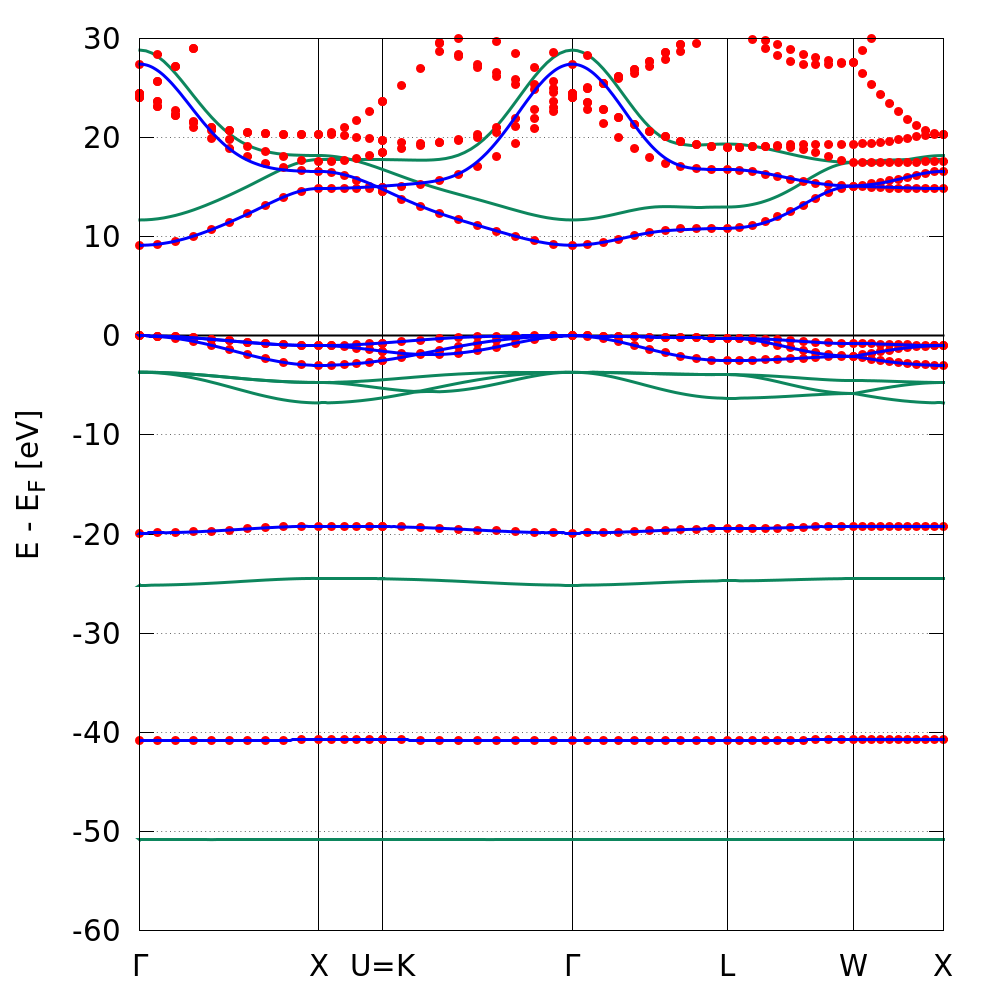
\includegraphics[width=0.5\linewidth]{LiF_kipz_bands.png}}
    %
    \vspace{1cm}
    %
    \begin{tabularx}{\linewidth}{*{3}{>{\centering\arraybackslash}X}}
        \hline
        \hline
        & MgO & LiF \\
        \hline
        occupied & Mg: $s$, $p$ / O: $s$, $p$ & Li: $s$, F: $s$, $p$ \\
        empty    & Mg: $s$ / O: $s$, $p$      & Li: $s$, F: $s$      \\
        \hline
    \end{tabularx}
    %
    \caption[KI and KIPZ band structures of MgO and LiF]{As per \cref{fig:bands-1-si-c-bn}, here we show the band structures of MgO and LiF obtained from the KI and KIPZ functionals.}
    \label{fig:bands-3-mgo-lif}
\end{figure}

In order to avoid ambiguity in the choice of MLWFs mixing different subspaces, we relied on the projected density-of-states to select the ``physically motivated'' initial projections. For covalent semiconductors like Si, C, Ge and GaAs, where the $s$ and $p$ orbitals contribute more or less equally in the energy range corresponding to the valence bands, the natural choice is that of $sp^3$ orbitals. In the case of GaAs and Ge, where $d$ semicore states are present, the Wannierization procedure gave rise to two sets of well distinguished groups of MLWFs ($d$-like and $sp^3$-bonding orbitals); however, for Ge we observed an unphysical mixing of the two types of orbitals. In this case, the two subsets of isolated valence bands were Wannierized separately in order to preserve the natural atomic character of the orbitals and to not mix Bloch functions corresponding to bands well separated in energy. This selection of the WFs follows also that of orbitalets used by Li \emph{et al.} \cite{li_localized_2018}, where the optimal orbitals are chosen via a localization procedure both in space and energy. A similar situation is observed in BN, MgO and LiF: $s$ and $p$ atomic orbitals contribute to separate ranges of energy and, for this reason, the hybridized choice $sp^3$ was considered ``less'' physical. In all cases, the KIPZ minimization reshapes the orbitals while maintaining the same atomic-like character.
\vspace{1cm}

We report in \crefrange{fig:bands-1-si-c-bn}{fig:bands-3-mgo-lif} the band structures for bulk Si, C-diamond, BN, Ge, GaAs, MgO, and LiF. The Koopmans correction is very smooth with respect to $\bk$, thereby applying an almost constant shift (different for each group of bands) to the KS-DFT bands. As a consequence, the major contribution to the dispersion of the energy in $\bk$-space comes from the DFT part; in order to distinguish between possible variations due to a flawed interpolation or effectively caused by the KC correction, we report also the interpolated DFT band structure. This has been obtained using the Wannier90 code, that applies the same interpolation method explained in \cref{sec:unfolding-method} to the DFT Hamiltonian only.

The calculated band gaps are reported in \cref{tab:gaps}, where we see that in most of the cases the agreement with the experiment is remarkable. In the case of diamond, all the Koopmans flavours significantly overestimate the gap of about 1~\ev. The reason might be related to the high degree of localization of the variational orbitals (see \cref{tab:sp3-sh}) that generally results in larger Koopmans corrections. We observe that, with respect to the other covalent semiconductors, the shift of the conduction bands of diamond is much larger. Using a different type of orbitals, e.g. starting from separate $s$- and $p$-like WFs, reduces the band gap, thanks to the smaller localization of the orbitals; however, this requires further study and justification, and it is not considered in this work. This case also unveils one of the limitations of the Koopmans approach: while the occupied variational orbitals are unambiguously defined as those that minimize the total energy, for the empty orbitals no analogous criterion exists. Here, the use of MLWFs represents a reasonable but nevertheless heuristic choice.

\begin{table}
    \centering
    \begin{tabularx}{\linewidth}{*{8}{>{\centering\arraybackslash}X}}
        \hline
        \hline
             &   PBE & QS$G\tilde{W}$ &    KI & pKIPZ &  KIPZ & Exp-ZPR &   ZPR \\
        \hline
        Si   &  0.55 &          1.24  &  1.23 &  1.22 &  1.24 &    1.22 &  $-0.05$ \\
        Ge   &  0.06 &          0.81  &  0.88 &  0.85 &  0.88 &    0.78 &  $-0.04$ \\
        GaAs &  0.50 &          1.61  &  1.58 &  1.54 &  1.55 &    1.57 &  $-0.05$ \\
        \hline
        C    &  4.16 &          5.90  &  6.84 &  6.87 &  6.94 &    5.86 &  $-0.36$ \\
        BN   &  4.52 &          6.59  &  7.25 &  7.09 &  7.15 &    6.62 &  $-0.42$ \\
        \hline
        MgO  &  4.73 &          8.30  &  8.87 &  8.68 &  9.04 &    8.47~\cite{shishkin_accurate_2007} &  $-0.64$ \\
        LiF  &  9.15 &         14.50  & 15.58 & 15.13 & 15.36 &   15.35~\cite{shishkin_accurate_2007} &  $-1.15$~\cite{nery_quasiparticles_2018} \\
        \hline
    \end{tabularx}
    \caption[Band gaps obtained with the finite-differences approach]{Fundamental band gaps (in \ev) as obtained from the three Koopmans flavours mentioned above, using the finite-differences approach. The values for Ge and GaAs are corrected by 0.1~\ev due to spin-orbit coupling. The QS$G\tilde{W}$ values are taken from Refs.~\cite{chen_accurate_2015,shishkin_accurate_2007}. If not specified otherwise, the experimental band gaps and the corresponding corrections due to zero-point renormalization (ZPR) are taken, respectively, from Refs. \cite{madelung_semiconductors_2004} and \cite{miglio_predominance_2020}. 
    }
    \label{tab:gaps}
\end{table}

\begin{table}[b]
    \centering
    \begin{tabularx}{\linewidth}{*{3}{>{\centering\arraybackslash}X}}
        \hline
        \hline
             & occupied & empty \\
        \hline
        Si   &    6.219         & 2.980         \\
        Ge   &    5.757         & 3.120         \\
        GaAs &    6.068         & 3.093         \\
        C    &    9.344         & 5.925         \\
        BN   &    8.407 / 7.714 & 4.681 / 5.313 \\
        \hline
    \end{tabularx}
    \caption[Hartree self-energies of the MLWFs of Si, Ge, GaAs, C, and BN]{Hartree self-energies (in \ev) of the (occupied and empty) MLWFs for the four covalent semiconductors and for BN.}
    \label{tab:sp3-sh}
\end{table}

For Si, Ge, GaAs and BN the agreement with previously published Koopmans results \cite{nguyen_koopmans-compliant_2018} is within 0.1~\ev. In the other cases the disagreement is probably due to the differences in the WFs used. We remark that, in Ref.~\cite{nguyen_koopmans-compliant_2018}, the whole procedure took place entirely within a supercell approach: the MLWFs were obtained from supercell $\Gamma$-sampling calculations where the additional degrees of freedom can give rise to qualitatively different Wannier functions. In fact, while in the supercell approach there is no constraint on the unitary transformation connecting Wannier and Bloch functions, in the primitive cell approach the unitary transformation is a block-diagonal (over $\bk$) matrix and so the mixing is different in the two approaches. This difference is even more marked when dealing with empty states: the presence of an entangled group of bands calls for a disentanglement procedure in order to define the Wannier functions, namely the selection of an optimal subset of Bloch states. This procedure is also $\bk$-dependent, thus the optimal set of Bloch functions selected in the supercell and primitive cell (even when the same energy windows are used) is generally different.

\begin{table}
    \centering
    \begin{tabularx}{\linewidth}{*{1}{>{\arraybackslash}>{\hsize=2.0\hsize}X}*{6}{>{\centering\arraybackslash}X}}
        \hline
        \hline
                                                 &   PBE &  QS$GW$ &    KI &  KIPZ &   Exp  \\
        \hline
        Si & & & & & \\
        $\Gamma_{1v} \rightarrow \Gamma'_{25v}$  & 11.96 & 12.04 & 11.96 & 12.09 & 12.5(6)  \\
        $X_{4v} \rightarrow \Gamma'_{25v}$       &  2.84 &  2.99 &  2.84 &  2.86 &  2.9     \\
        $L_{1v} \rightarrow \Gamma'_{25v}$       &  6.96 &  7.18 &  6.96 &  7.04 &  6.8(2)  \\
        $L'_{2v} \rightarrow \Gamma'_{25v}$      &  9.63 &  9.79 &  9.63 &  9.74 &  9.3(4)  \\
        \\
        $\Gamma'_{25v} \rightarrow \Gamma_{15c}$ &  2.56 &  3.35 &  3.24 &  3.26 &  3.35(1) \\
        $\Gamma'_{25v} \rightarrow \Gamma'_{2c}$ &  3.33 &  4.08 &  4.00 &  4.01 &  4.15(1) \\
        $\Gamma'_{25v} \rightarrow X_{1c}$       &  0.69 &  1.44 &  1.36 &  1.37 &  1.13    \\
        $\Gamma'_{25v} \rightarrow L_{1c}$       &  1.51 &  2.27 &  2.18 &  2.19 &  2.04(6) \\
        $\Gamma'_{25v} \rightarrow L_{3c}$       &  3.33 &  4.24 &  3.99 &  4.00 &  3.9(1)  \\
        \hline
        GaAs & & & & & \\
        $\braket{\varepsilon_d}$                 & 14.9  & 17.6  & 16.9  & 17.7  & 18.9     \\
        \hline
        LiF & & & & & \\
        $\braket{\varepsilon_{1s({\rm Li})}}$    & 40.8  &  --   & 46.2  & 47.1  & 49.8     \\
        $\braket{\varepsilon_{2s({\rm F})}}$     & 19.5  &  --   & 20.2  & 21.0  & 23.9     \\
        \hline
    \end{tabularx}
    \caption[Intra-band and inter-band transition energies of Si; deep bands of GaAs and LiF]{In the upper part we report the energy differences (in \ev) for Si at special symmetry points in the BZ, wrt to the top of the valence band ($\Gamma'_{25v}$). The results from $GW$ calculations and the experimental values are taken, respectively, from Refs.~\cite{hybertsen_electron_1986} and \cite{madelung_semiconductors_2004}. The central part of the table contains the average position of the $d$-bands of GaAs; in this case the experimental and theoretical (self-consistent $GW$) values are taken from Ref.~\cite{shishkin_accurate_2007}. At the bottom we report the position of the $1s$ bands of Li and $2s$ bands of F in LiF; experimental values are taken from Ref.~\cite{johansson_core_1976}.}
    \label{tab:ene-special-points}
\end{table}

With regard to the rest of the spectrum, by looking at \crefrange{fig:bands-1-si-c-bn}{fig:bands-3-mgo-lif} we see that the main effect of the Koopmans correction is a shift of the DFT band groups -- downward for the valence, upward for the conduction -- quite smoothly with respect to $\bk$, and fairly constant for bands corresponding to orbitals with the same chemical character. In principle, the only situation where the correction consists of a rigid shift of the bands is for the case of the KI potential acting on equivalent occupied states. From \cref{eq:ki-pot-occ}, we know that the KI potential for the occupied states is scalar, thus its representation on the variational orbitals yields a diagonal matrix. When the occupied orbitals have all the same character, which is for instance the case of the $sp^3$ orbitals in Si or C, the KI potential reduces to a multiple of the identity and the correction is a simple shift applied to all the DFT eigenvalues. On the other hand, in the presence of valence orbitals with a different character -- e.g. $sp^3$ and $d$ orbitals in GaAs -- although still diagonal, the KI potential is not anymore a multiple of the identity matrix and the effect of the correction is non-trivial. This becomes even more pronounced for the potential acting on the empty states or for the KIPZ potential: because of the presence of space-dependent terms, the matrix representation of the potential is non-diagonal and the Koopmans correction can affect also the bandwidth as well as the inter- and intra-band distances. Yet, the effect of these off-diagonal elements is minor: in a localized representation, such as that of the variational orbitals, and because of the local nature of the Koopmans Hamiltonian, the dominant matrix elements are diagonal, whereas the contribution from the off-diagonal matrix elements is second-order.

Finally, in \cref{tab:ene-special-points} we can see that for Si the relative distance between valence bands (first block of points), well described already at the PBE level, is not modified by the KI correction. The second block of points shows the energies which are different from the fundamental band gap: the remarkable agreement with the results from photoemission experiments, and not only with the first ionization energies, further emphasizes the capability of KC functionals in predicting the full band structure.

\subsection{DFPT\label{sec:results-dfpt}}
Here, we report the results obtained with the PC implementation of the KI functional for two systems: gallium arsenide and zinc oxide \cite{colonna_koopmans_2022}. The first system allows for a comparison between the finite-differences approach, which uses the full expressions of $\Pi_i^{\rm KI}$ [given by \cref{eq:ki-correction} and the linear response approach, based on a second-order approximation of the KI correction terms [given by \cref{eq:relaxed-ki-second-order}]. The second system instead highlights the advantages of this recently developed PC-based implementation, which makes more feasible to deal with complex systems: the PC of ZnO contains about 2 to 3 times more (pseudo-)electrons than the previously considered systems which, in the SC approach, brings to an increased computational load of one to two orders of magnitudes (for the supercells considered in this work).

\begin{figure}
    \centering
    %
    \subfloat[]{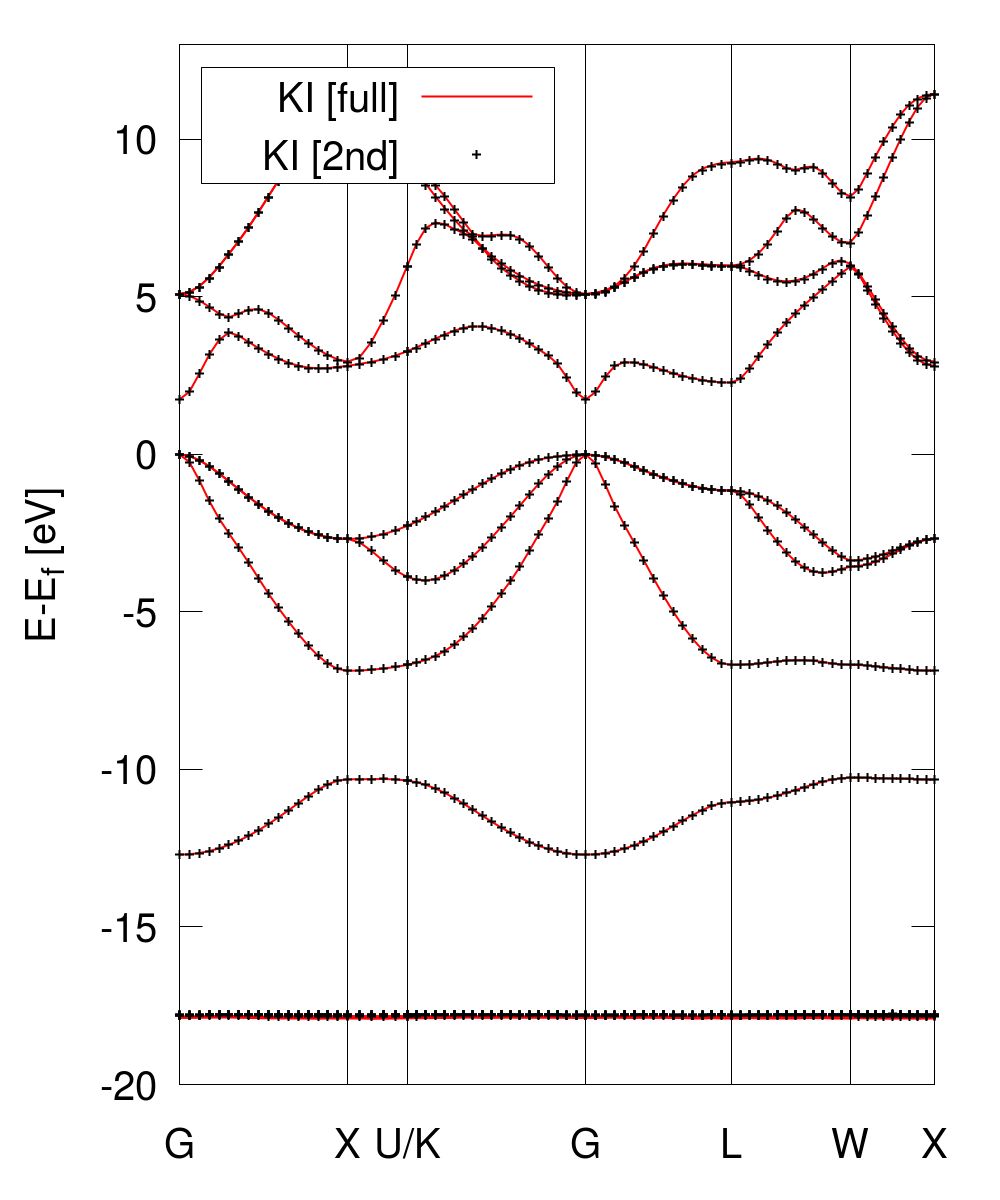
\includegraphics[width=0.5\linewidth]{GaAs_full_vs_2nd_LDA.png}}
    \subfloat[]{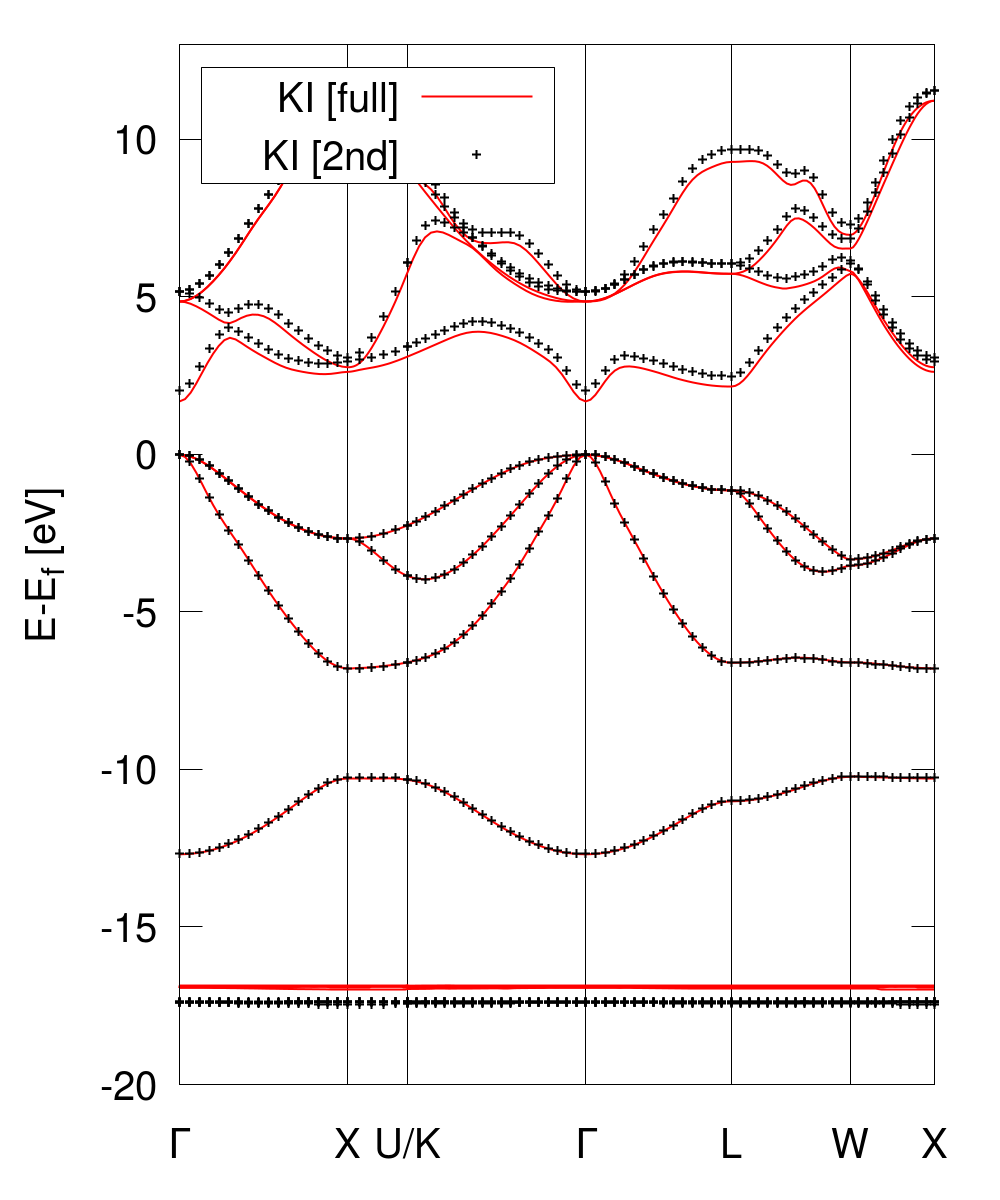
\includegraphics[width=0.5\linewidth]{GaAs_full_vs_2nd_PBE.png}}
    %
    \vspace{5mm}
    %
    \begin{tabularx}{0.8\linewidth}{*{1}{>{\arraybackslash}>{\hsize=2cm}X}*{2}{>{\centering\arraybackslash}X}}
        \hline
        \hline
        & LDA & PBE \\
        & \hfill $E_{\rm g}$ \hfill $\braket{\varepsilon_d}$ \hfill\null
        & \hfill $E_{\rm g}$ \hfill $\braket{\varepsilon_d}$ \hfill\null \\
        \hline
        KI full & \hfill 1.74 \hfill -17.8 \hfill\null & \hfill 1.68 \hfill -16.9 \hfill\null \\
        KI 2nd  & \hfill 1.75 \hfill -17.8 \hfill\null & \hfill 2.02 \hfill -17.4 \hfill\null \\
        \hline
    \end{tabularx}
    %
    \vspace{5mm}
    %
    \caption[Comparison finite-differences and linear response methods: band structure of GaAs]{KI band structure of GaAs as calculated with the (full) finite-differences and the (second-order) linear response approach, using (a) LDA-based and (b) PBE-based functionals. At the bottom we report the numerical results (in \ev) for the band gap (for the sake of comparison, we did not include any renormalizations due to zero-point motion and spin-orbit coupling) and for Ga $d$-bands.}
    \label{fig:comparison-gaas-dscf-dfpt}
\end{figure}

In \cref{fig:comparison-gaas-dscf-dfpt}, we report the band structure of GaAs as obtained from the two approaches, using an identical setup (same MLWFs and same parameters). When applying the KI correction on top of the LDA functional, the second-order approximation does not seem to affect results -- this is not always the case, as there are systems, such as LiF, for which the second-order approximation of KI@LDA deviates from the full functional, as showed in Ref.~\cite{colonna_koopmans_2022} -- whereas when starting from PBE there are significative differences in the empty bands, as well as in the deep flat bands coming from the $d$-states of Ga. The second-order approximation brings to different expressions for the screening parameters and for the Koopmans Hamiltonian which, in principle, could become significant for systems that are not dominated by the Hartree and self-Hartree terms -- we recall that the Hartree energy depends quadratically on the density and, therefore, it is exact at the second-order. For such systems the contribution from the exchange-correlation energy, as well as from the orbital xc self-energies, could become important and the truncation of such terms could lead to the discrepancies described above. Understanding whether such differences impact more the screening parameters, or the Koopmans Hamiltonian (or both), is not trivial and definitely deserves some further investigations. Yet, the possibility of performing self-consistent calculations using approximation-free Koopmans functionals in any flavors, highlights the importance of the \kcp implementation.

\begin{figure}
    \centering
    %
    \subfloat[]{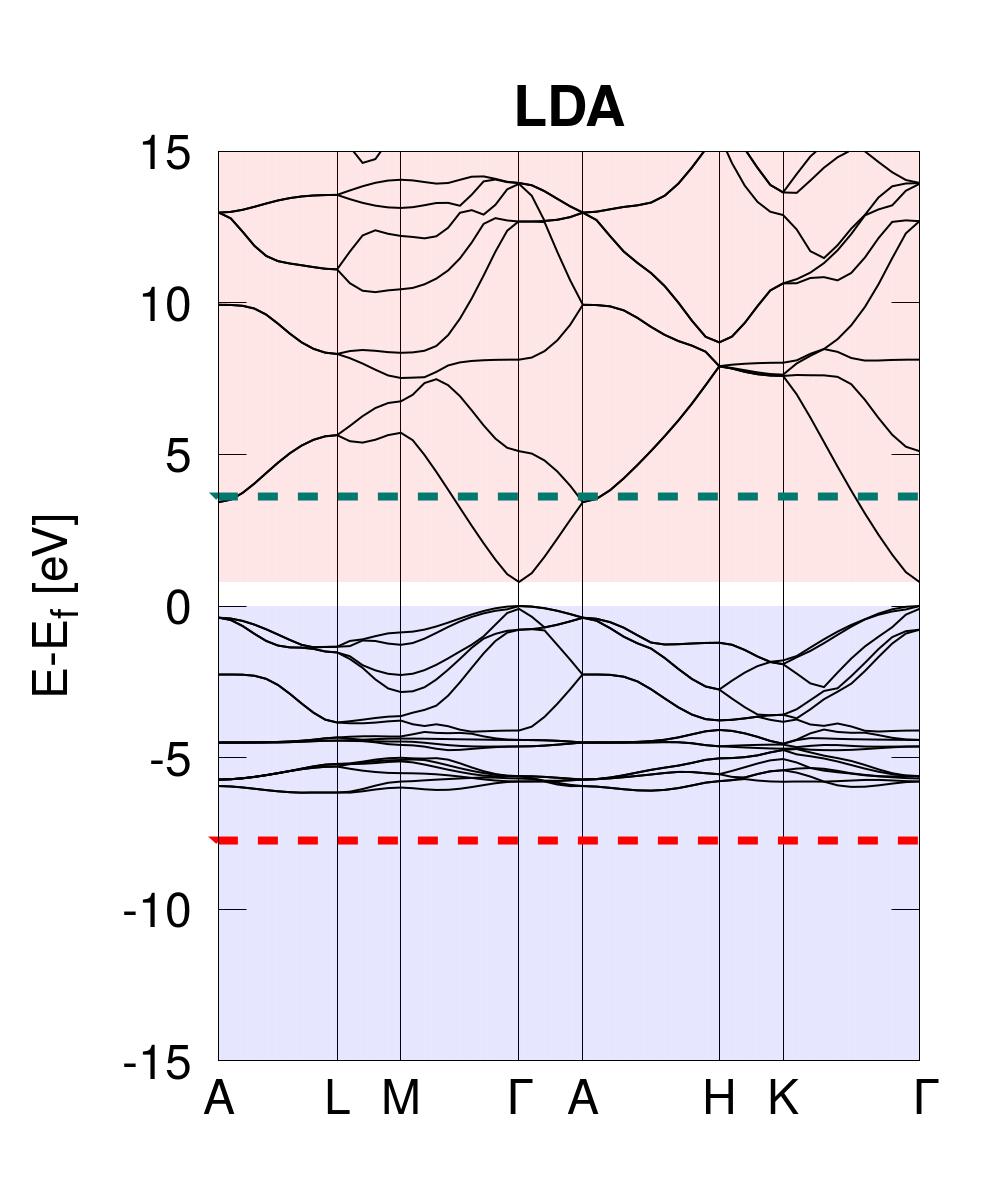
\includegraphics[width=0.33\linewidth]{ZnO_lda.png}}
    \subfloat[]{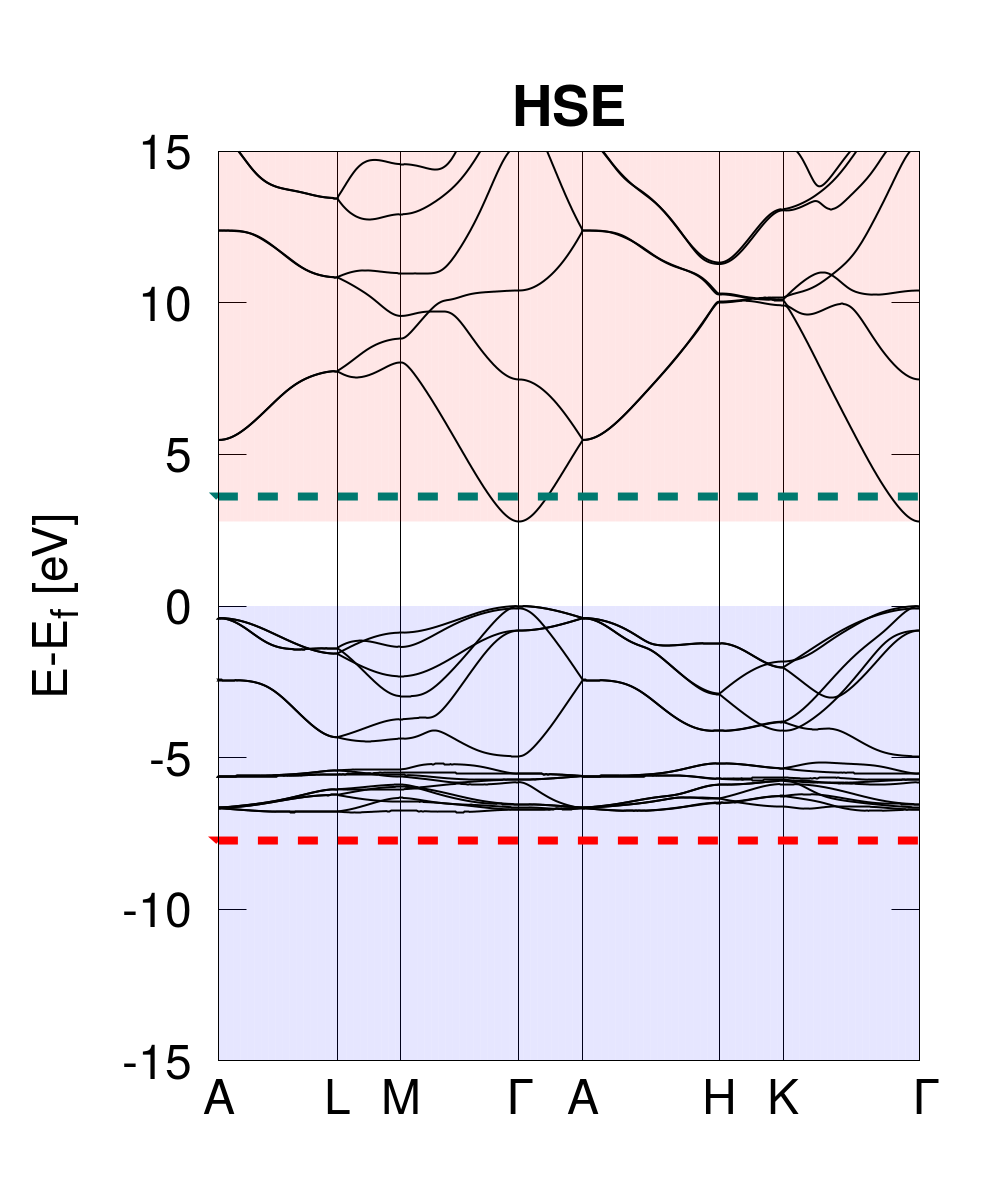
\includegraphics[width=0.33\linewidth]{ZnO_hse.png}}
    \subfloat[]{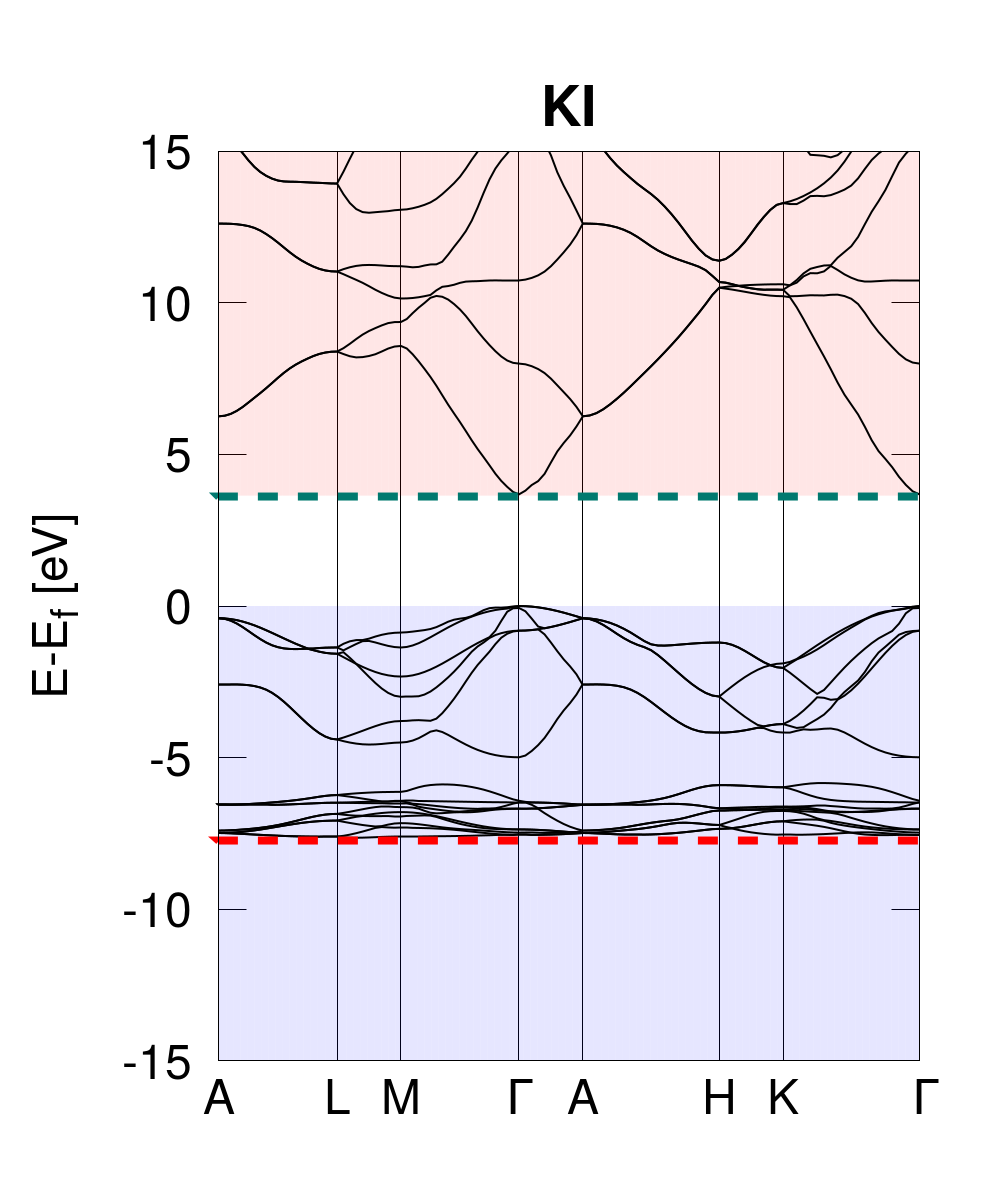
\includegraphics[width=0.33\linewidth]{ZnO_ki.png}}
    %
    \vspace{3mm}
    %
    \begin{tabularx}{0.9\linewidth}{*{1}{>{\arraybackslash}>{\hsize=1cm}X}*{6}{>{\centering\arraybackslash}X}}
        \hline
        \hline
                                 &  LDA &  HSE & $GW_0$ & sc$G\tilde{W}$ &   KI &  Exp \\
        \hline
        $E_{\rm g}$              & 0.79 & 2.79 &    3.0 &            3.2 & 3.62 & 3.60 \\
        $\braket{\varepsilon_d}$ & -5.1 & -6.1 &   -6.4 &           -6.7 & -6.9 & -7.5/8.0 \\
        \hline
    \end{tabularx}
    %
    \vspace{3mm}
    %
    \caption[Band structure of ZnO]{Band structure of ZnO calculated at different level of theory: LDA (left panel), HSE (middle panel) and KI (right panel). Shaded areas highlight valence (light blue) and conduction (light red) manifolds. The experimental values for the band gap and for the energy position of 
    Zn $d$-states are represented by the dashed green line and by the dashed red line, respectively. In the table we report the values for the band gap and for the average position of the Zn $d$-bands. As in \cref{tab:gaps}, we subtracted the ZPR (-0.16~\ev for ZnO \cite{cardona_isotope_2005}) to the experimental band gap. \gw and experimental values were taken from Ref.~\cite{shishkin_accurate_2007}.}
    \label{fig:bands-zno}
\end{figure}

Zinc oxide is a transition metal oxide which, at ambient conditions, crystallizes in a hexagonal wurtzite structure; it is well known that ZnO is a challenging system for Green's function theory~\cite{shih_quasiparticle_2010,samsonidze_insights_2014}, thus it represents a particularly relevant system for Koopmans functionals. In \cref{fig:bands-zno}, we show the band structure calculated at different levels of theory together with a comparison with experimental results. The bands around the gap are dominated by the oxygen $2p$ states in the valence, and the Zn $4s$ states in the conduction with some contribution from O $2p$ and $2s$. At LDA level, the band gap is dramatically underestimated when compared to the experimental value. This underestimation is even more severe than in semiconductors with similar electronic structure and band gap, like e.g. GaN, and has been related to the repulsion and hybridization of the oxygen $p$- and zinc $d$-states \cite{wei_role_1988, lim_angle-resolved_2012}. In fact, at LDA level, the bands coming from Zn $d$-states lie below the O $2p$ valence bands, but are too high in energy, resulting in upwards repulsion of the valence band maximum, and in an exaggerated reduction of the band gap \cite{lim_angle-resolved_2012}. Here, we also compared the band structure calculated from the HSE hybrid functional, which pushes the $d$-states down in energy and opens up the band gap improving the agreement with the experimental values. The KI functional moves in the same direction and further reduces the discrepancies with the experiment, providing an overall satisfactory description of the electronic structure, in excellent agreement with the experiment.

It is important to mention that in this case a different choice was made for the non-self-consistent variational orbitals, represented by the so-called \emph{projected Wannier functions}. These are the WFs resulting from the projection (and the reorthonormalization) of the KS states onto the provided initial atomic-like orbitals and, for the empty states, from the additional -- and, usually, unavoidable -- disentanglement procedure. No minimization of the spread functional is then applied, which allows obtaining WFs that reflect the atomic-like character of the bands. This choice is actually consistent with the strategy discussed in \cref{sec:results-dscf} for the construction of the WFs: if on one hand they should be as localized as possible, in order to have non-trivial Koopmans corrections, on the other they should not spread excessively in the energy domain. In ZnO, as a consequence of the entanglement of valence bands with different atomic characters, the maximal localization procedure brings about an unwanted mixing, or hybridization, of the KS states and a consequent deterioration of the results. Besides, we highlight that the WFs resulting from the simple projection of the KS states are already sufficiently localized to have effective Koopmans corrections.

\section{Conclusions\label{sec:results-conclusions}}
Koopmans spectral functionals showed remarkable results for the prediction of the quasiparticle energies of crystalline periodic systems, proving to be one of the best methods for electronic band structure calculations. The finite-differences SC-based approach allows performing fully self-consistent calculations with any flavors of Koopmans functionals, although it requires an unfolding procedure to reconstruct the band structure within the BZ. On the other hand, the linear response PC-based approach allows for KI calculations on top of (maximally localized) Wannier functions, while resorting to a second-order approximation of the KI correction terms. Such approximation showed, in some cases, discrepancies with the full approach which can be traced back to the different expressions for the screening parameters and for the Koopmans Hamiltonian, and definitely deserve more attention. The greater simplicity and computational feasibility of this approach with respect to Green's function-based methods, together with the high accuracy of KI results (comparable to state-of-the-art MBPT methods), makes \kcw an ideal candidate for large-scale band structure calculations. Moreover, given the recent developments in the automatization of the Wannierization procedure \cite{vitale_automated_2020,qiao_wannier_2022}, \kcw could be coupled to these methods and provide a reliable and efficient tool for high-throughput band structure calculations. Besides, the \kcp implementation remains the most rigorous approach, as it overcomes the errors due to the second-order approximation and supports KIPZ calculations too, and it should be preferred whenever the circumstances demand for calculations with Koopmans functionals at the best of their possibilities.

All the information and the data needed to reproduce the results discussed in this chapter, can be found on the Materials Cloud Archive \cite{de_gennaro_blochs_mc_2022,colonna_koopmans_mc_2021}.

